%=====================================================================
% TRABALHO DE CONCLUSÃO DE CURSO (TCC)
% Universidade Federal de Santa Catarina (UFSC)
% Título: Reconhecimento de Texto em Imagens de Obras Literárias 
%         Antigas em Português
% Autor: Ewaldo Uhlmann
% Orientador: Prof. Dr. Renato Fileto
% Ano: 2026
%=====================================================================

\documentclass[
  12pt,
  oneside,
  a4paper,
  chapter=TITLE,
  section=TITLE,
  english,
  brazil
]{abntex2}

%=====================================================================
% PACOTES ESSENCIAIS
%=====================================================================
\usepackage[T1]{fontenc}
\usepackage[utf8]{inputenc}
\usepackage{lmodern}
\usepackage{indentfirst}
\usepackage{graphicx}
\usepackage{amsmath}
\usepackage{amssymb}
\usepackage{hyperref}
\usepackage{microtype}
\usepackage{xcolor}
\usepackage{float}
\usepackage{placeins}
\usepackage[num]{abntex2cite}

\newcommand{\attention}[1]{{\color{red}#1}}
\newcommand{\propFileto}[1]{\textcolor{blue}{#1}}
\newcommand{\propEwaldo}[1]{\textcolor{black}{#1}}

%=====================================================================
% COMANDO CUSTOMIZADO PARA TÓPICOS A COMPLETAR
%=====================================================================
\newcommand{\topic}[1]{\textit{\textcolor{gray}{[TODO: #1]}}}

%=====================================================================
% CONFIGURAÇÕES DE APARÊNCIA
%=====================================================================
\makeatletter
\hypersetup{
    pdftitle={\@title}, 
    pdfauthor={\@author},
    pdfsubject={\imprimirpreambulo},
    pdfcreator={LaTeX with abntex2},
    colorlinks=true,
    linkcolor=black,
    citecolor=black,
    filecolor=magenta,
    urlcolor=blue,
    bookmarksdepth=4
}
\makeatother

%=====================================================================
% INFORMAÇÕES DO TRABALHO
%=====================================================================
\titulo{Reconhecimento de Texto em Imagens de Obras Literárias Antigas em Português}

\autor{Ewaldo Uhlmann}

\orientador{Prof. Dr. Renato Fileto}

\local{Florianópolis}

\data{2026}

\instituicao{Universidade Federal de Santa Catarina \par Centro Tecnológico \par
Departamento de Informática e Estatística}

\tipotrabalho{Trabalho de Conclusão de Curso}

\preambulo{Trabalho de Conclusão de Curso submetido ao Curso de Graduação em Ciências
da Computação da Universidade Federal de Santa Catarina para a obtenção do Grau de
Bacharel em Ciências da Computação.}

%=====================================================================
% AJUSTES DE ESPAÇAMENTO
%=====================================================================
\setlength{\parindent}{1.3cm}
\setlength{\parskip}{0.2cm}

%=====================================================================
% INÍCIO DO DOCUMENTO
%=====================================================================
\begin{document}

\selectlanguage{brazil}
\frenchspacing
\OnehalfSpacing

%=====================================================================
% ELEMENTOS PRÉ-TEXTUAIS
%=====================================================================

\imprimircapa

\imprimirfolhaderosto

\begin{folhadeaprovacao}
  \begin{center}
    {\ABNTEXchapterfont\large\imprimirautor}
    \vspace*{\fill}\vspace*{\fill}
    \begin{center}
      \ABNTEXchapterfont\bfseries\Large\imprimirtitulo
    \end{center}
    \vspace*{\fill}
    \hspace{.45\textwidth}
    \begin{minipage}{.5\textwidth}
        \imprimirpreambulo
    \end{minipage}%
    \vspace*{\fill}
   \end{center}
   \begin{center}
   Este trabalho foi julgado adequado para obtenção do Título de Bacharel em
   Ciências da Computação e aprovado em sua forma final pela banca examinadora.
   \end{center}
   \vspace*{\fill}
   \begin{center}
     Florianópolis, 30 de Abril de 2026
   \end{center}
\end{folhadeaprovacao}

%---------------------------------------------------------------------
% RESUMO
%---------------------------------------------------------------------
\begin{resumo}

Este trabalho investiga a aplicação de técnicas de reconhecimento óptico de caracteres
(OCR) em obras literárias históricas em português pertencentes ao acervo do NUPILL
(Núcleo de Pesquisas em Informática, Literatura e Linguística da UFSC). Para isso,
são revisados fundamentos, métodos, benchmarks e estudos comparativos existentes na
literatura, bem como as principais ferramentas de OCR disponíveis, cobrindo desde
abordagens clássicas até modelos modernos baseados em aprendizado profundo e
visão-linguagem. As ferramentas mais promissoras são então avaliadas comparativamente
sobre um corpus de páginas de obras históricas selecionadas e transcritas manualmente,
cobrindo distintos níveis de dificuldade tipográfica e de degradação física. Com base
nos resultados obtidos, seleciona-se a ferramenta mais adequada ao contexto, que é
então empregada na extração e transcrição completa de uma obra do acervo. O processo
é estruturado na forma de um pipeline replicável, acompanhado de diretrizes
metodológicas que visam orientar iniciativas similares de digitalização de acervos
históricos em português.

\vspace{\onelineskip}

\noindent
\textbf{Palavras-chave}: reconhecimento óptico de caracteres; obras literárias
históricas; literatura brasileira; avaliação comparativa de ferramentas;
digitalização de acervos.

\end{resumo}

%---------------------------------------------------------------------
% ABSTRACT
%---------------------------------------------------------------------
\begin{resumo}[Abstract]
\selectlanguage{english}

This work investigates the application of Optical Character Recognition (OCR) techniques
to historical literary works in Portuguese from the NUPILL collection (Núcleo de
Pesquisas em Informática, Literatura e Linguística, UFSC). To this end, existing
benchmarks and comparative studies from the literature are reviewed, along with the
main OCR tools and approaches available, ranging from classical methods to modern
deep learning and vision-language models. The most promising tools are then
comparatively evaluated on a corpus of manually transcribed pages covering varying
levels of typographic complexity and physical degradation. Based on the results, the
most suitable tool is selected and applied to the full extraction and transcription of
a work from the collection. The process is structured as a replicable pipeline,
accompanied by methodological guidelines intended to support similar digitization
initiatives for historical documents in Portuguese.

\vspace{\onelineskip}

\noindent
\textbf{Keywords}: optical character recognition; historical literary works; Brazilian
literature; comparative tool evaluation; document digitization.

\end{resumo}

\selectlanguage{brazil}

%---------------------------------------------------------------------
% AGRADECIMENTOS
%---------------------------------------------------------------------
%\begin{agradecimentos}

%\topic{Agradecimentos ao Prof.\ Dr.\ Renato Fileto pela orientação, ao
%Prof.\ Dr.\ Alckmar Luiz dos Santos pela colaboração com o NUPILL, aos colegas que
%contribuíram com sugestões e feedback, e à comunidade de pesquisa em Humanidades
%Digitais.}

%\end{agradecimentos}

%---------------------------------------------------------------------
% LISTAS E SUMÁRIO
%---------------------------------------------------------------------
\pdfbookmark[0]{\listfigurename}{lof}
\listoffigures*
\cleardoublepage

\pdfbookmark[0]{\listtablename}{lot}
\listoftables*
\cleardoublepage

\pdfbookmark[0]{\contentsname}{toc}
\tableofcontents*
\cleardoublepage

%=====================================================================
% ELEMENTOS TEXTUAIS
%=====================================================================
\textual

%=====================================================================
% CAPÍTULO 1: INTRODUÇÃO
%=====================================================================
\chapter{Introdução}

A preservação do patrimônio literário histórico representa um desafio relevante para
a manutenção da memória cultural e para a disponibilização de fontes primárias à
comunidade acadêmica. No caso específico da literatura brasileira do século XIX e XX,
muitos textos de importância histórica e intelectual encontram-se em estado físico
deteriorado, com acesso restrito ou disponíveis apenas em acervos especializados. A
digitalização automatizada dessas obras é uma estratégia que permite não apenas a
preservação de seu conteúdo, mas também a democratização do acesso e a viabilização
de análises computacionais em larga escala.

O reconhecimento óptico de caracteres (OCR --- \textit{Optical Character Recognition})
emerge como a tecnologia fundamental para transformar imagens de documentos em texto
editável e processável. Contudo, o desempenho de sistemas OCR varia significativamente
em função das características físicas dos documentos, da qualidade da digitalização e
das particularidades linguísticas do texto. Documentos históricos apresentam desafios
específicos: degradação do papel, variações tipográficas características da época,
entintamento desigual, e, no caso do português, a presença de diacríticos e de
vocabulário arcaico.
Apesar da disponibilidade de ferramentas de reconhecimento óptico de caracteres (OCR),
ainda há pouca sistematização sobre como aplicá-las de forma eficaz em documentos
antigos em português, especialmente aqueles que apresentam degradação física, variações tipográficas e ortografia não padronizada \cite{clausner2011}.



\section{Contextualização e Justificativa}

Universidades brasileiras e outras instituições vêm ampliando esforços para digitalizar
acervos históricos, buscando não apenas preservar obras antigas, mas também torná-las
acessíveis para novas formas de pesquisa \cite{terras2013}. O
NUPILL\footnote{\url{https://nupill.ufsc.br/}} (Núcleo de Pesquisas em Informática,
Literatura e Linguística) da Universidade
Federal de Santa Catarina (UFSC) é um exemplo desse movimento, atuando na interseção
entre tecnologia e estudos literários.
O NUPILL dedica-se ao estudo de acervos literários históricos,
combinando abordagens da literatura com métodos computacionais. Como parte de seus
objetivos, o NUPILL busca digitalizar e disponibilizar obras 
para a pesquisa em Humanidades Digitais.
A conversão de documentos para texto digital não se limita à preservação, mas
também viabiliza novas formas de uso, como busca textual, indexação e análises em larga
escala \cite{burdick2012}, ampliando significativamente o potencial de pesquisa.


Dentro desse contexto, obras literárias do século XIX presentes no acervo do NUPILL
ilustram bem os desafios envolvidos. Esses materiais frequentemente apresentam
degradação física, variações tipográficas e ortografia não padronizada, o que dificulta
sua digitalização por métodos tradicionais.
Do ponto de vista tecnológico, o OCR evoluiu significativamente nos últimos anos.
Modelos baseados em arquiteturas de Transformers, como o TrOCR, têm apresentado
desempenho superior em diversas tarefas de reconhecimento de texto \cite{huang2021}.
Ainda assim, existe uma lacuna importante: pouco se sabe sobre o comportamento desses
modelos quando aplicados a textos históricos em português, especialmente aqueles do
século XIX \cite{smith2019}.

Este trabalho se insere no contexto da digitalização de documentos antigos como presentes no acervo do NUPILL. O objetivo não é apenas digitalizar um corpus
específico, mas compreender e documentar o processo de aplicação de técnicas de OCR
nesse contexto, de forma que o processo a ser desenvolvido neste trabalho possa ser replicado e adaptado para outras obras literárias.

\section{Objetivos}

O objetivo geral deste trabalho é investigar a aplicação de técnicas e ferramentas para reconhecimento óptico de
caracteres (OCR) em obras literárias antigas em português, avaliando diferentes
alternativas e identificando aquela mais adequada para esse contexto, além de estruturar
um processo que possa ser aplicado ao acervo do NUPILL.

\section{Objetivos Específicos}

\begin{enumerate}
    \item Efetuar uma revisão bibliográfica sobre técnicas e ferramentas de OCR que
    possam ser aplicadas a textos históricos.

    \item Avaliar diferentes ferramentas de OCR por meio de testes em amostras
    representativas de obras literárias históricas.

    \item Construir um conjunto de referência (\textit{ground truth}) por meio de
    transcrição manual de uma amostra representativa do corpus, a ser utilizado como
    base para a escolha do modelo.

    \item Comparar o desempenho dos modelos considerando métricas de qualidade (como
    CER e WER), além de aspectos práticos como custo computacional, custo financeiro e
    facilidade de uso.

    \item Selecionar a ferramenta mais adequada para o reconhecimento de obras
    literárias históricas em português.

    \item Desenvolver e configurar um pipeline de extração automática de texto
    aplicável ao acervo do NUPILL.

    \item Aplicar o pipeline em um conjunto de documentos, analisando os resultados
    obtidos.

    \item Identificar limitações, padrões de erro e desafios recorrentes no processo de
    OCR em obras literárias históricas.

    \item Documentar o processo e propor recomendações para sua reutilização em outros
    projetos semelhantes.
\end{enumerate}

\section{Delimitação do Estudo}

Este trabalho concentra-se na avaliação e aplicação de técnicas de reconhecimento
óptico de caracteres (OCR) em obras literárias históricas em português, com foco em
materiais que apresentam características como degradação física, variações tipográficas
e ortografia não padronizada, típicas de publicações do século XIX.

A pesquisa limita-se à análise de modelos de OCR já existentes, incluindo abordagens
clássicas e baseadas em aprendizado profundo, não contemplando o desenvolvimento ou
treinamento de novos modelos a partir do zero. O objetivo é compreender o desempenho
dessas soluções no contexto específico estudado e identificar aquela mais adequada.

Além disso, o estudo considera um conjunto representativo de obras como base
experimental, não abrangendo a totalidade do acervo do NUPILL. A implementação de um
pipeline de extração de texto é realizada com foco em reprodutibilidade e adaptação,
mas sem a pretensão de resolver todos os desafios associados ao OCR em obras literárias
históricas.

Por fim, aspectos como pós-processamento avançado de texto, correção linguística
automatizada em larga escala e análise semântica aprofundada não fazem parte do escopo
deste trabalho, podendo ser explorados em pesquisas futuras.

\section{Contribuições Esperadas}

Espera-se que este trabalho contribua para a compreensão do uso de técnicas de OCR em
obras literárias antigas em português, fornecendo uma análise comparativa entre
diferentes ferramentas disponíveis.

Como principal contribuição, busca-se auxiliar na escolha de modelos de OCR mais
adequados para esse tipo de material, considerando não apenas a qualidade do
reconhecimento, mas também fatores práticos como custo computacional, custo financeiro
e facilidade de integração.

Além disso, o trabalho propõe a estruturação de um processo de extração automática de
texto que possa ser reutilizado em iniciativas de digitalização de acervos, contribuindo
para a automação da conversão de obras físicas em formatos digitais processáveis.

Por fim, espera-se identificar limitações, padrões de erro e desafios recorrentes nesse
contexto, oferecendo recomendações que possam orientar aplicações futuras no âmbito do
NUPILL e de projetos semelhantes.

\section{Organização do Documento}

Este trabalho está estruturado em oito capítulos, organizados da seguinte forma:

\begin{itemize}
    \item \textbf{Capítulo 1 -- Introdução:} apresenta a contextualização do problema,
    os objetivos, a delimitação do estudo e as contribuições esperadas.

    \item \textbf{Capítulo 2 -- Fundamentação Teórica:} discute os conceitos
    relacionados ao reconhecimento óptico de caracteres e os desafios associados a obras
    literárias históricas.

    \item \textbf{Capítulo 3 -- Trabalhos Relacionados:} apresenta pesquisas e
    iniciativas relevantes na área de OCR e digitalização de acervos.

    \item \textbf{Capítulo 4 -- Construção da Regra Ouro:} descreve a composição do
    corpus de avaliação e o processo de transcrição manual utilizado como referência.

    \item \textbf{Capítulo 5 -- Metodologia Experimental:} descreve as etapas de
    avaliação, seleção de modelos e implementação do pipeline de processamento.

    \item \textbf{Capítulo 6 -- Implementação e Resultados:} apresenta a implementação
    desenvolvida e os resultados obtidos, incluindo análises quantitativas e qualitativas.

    \item \textbf{Capítulo 7 -- Discussão:} analisa os resultados, destacando
    limitações, implicações práticas e possíveis melhorias.

    \item \textbf{Capítulo 8 -- Conclusão:} retoma os principais achados do trabalho e
    apresenta sugestões para trabalhos futuros.
\end{itemize}

%=====================================================================
% CAPÍTULO 2: FUNDAMENTAÇÃO TEÓRICA
%=====================================================================
\chapter{Fundamentação Teórica}

A fundamentação teórica deste trabalho estabelece os conceitos essenciais para
compreender o reconhecimento óptico de caracteres em obras literárias históricas. Este
capítulo apresenta os princípios técnicos de OCR, as principais técnicas e ferramentas
avaliadas, as métricas de avaliação utilizadas e os desafios específicos enfrentados na
digitalização de obras antigas em português.

%---------------------------------------------------------------------
\section{Reconhecimento Óptico de Caracteres (OCR)}
%---------------------------------------------------------------------

O Reconhecimento Óptico de Caracteres (OCR) é a tecnologia que transforma imagens de
texto em formatos legíveis por máquina, permitindo a conversão de documentos impressos
ou manuscritos em texto digital editável e processável \cite{OneAdvanced2022}.
Historicamente, a tecnologia tem raízes profundas: em 1914, o físico Emanuel Goldberg
inventou uma máquina que podia ler caracteres e convertê-los em código telegráfico,
marcando um dos primeiros passos da OCR \cite{Incode2025}.

\subsection{Evolução Histórica do OCR}

A evolução da OCR ocorreu em várias etapas bem definidas. Nos anos 1950, as primeiras
aplicações comerciais de OCR surgiram nos setores bancário e postal. Um marco importante
foi em 1974, quando Ray Kurzweil fundou a Kurzweil Computer Products e desenvolveu o
primeiro sistema OCR omni-fonte, capaz de reconhecer texto impresso em praticamente
qualquer fonte \cite{Incode2025}. Durante os anos 1980 e 1990, o foco deslocou-se para
o desenvolvimento de algoritmos mais sofisticados, permitindo o reconhecimento de
múltiplas fontes e línguas.

A virada do milênio trouxe uma transformação significativa: a integração de inteligência
artificial (IA) e aprendizado de máquina (AM) aos sistemas OCR \cite{Idenfo2024}. Isso
permitiu que o OCR processasse tipos de documentos mais diversos com maior precisão.
Atualmente, a tecnologia continua evoluindo, com modelos baseados em aprendizado profundo
(\textit{deep learning}) e arquiteturas de Transformer apresentando resultados sem
precedentes \cite{PictureText2025}.

\subsection{O Pipeline de um Sistema OCR}

Um sistema de reconhecimento óptico de caracteres segue um processo sequencial bem
definido, no qual cada etapa constrói sobre o resultado da etapa anterior. A
Figura~\ref{fig:ocr_pipeline} ilustra as principais fases deste processo.

\begin{figure}[H]
    \centering
    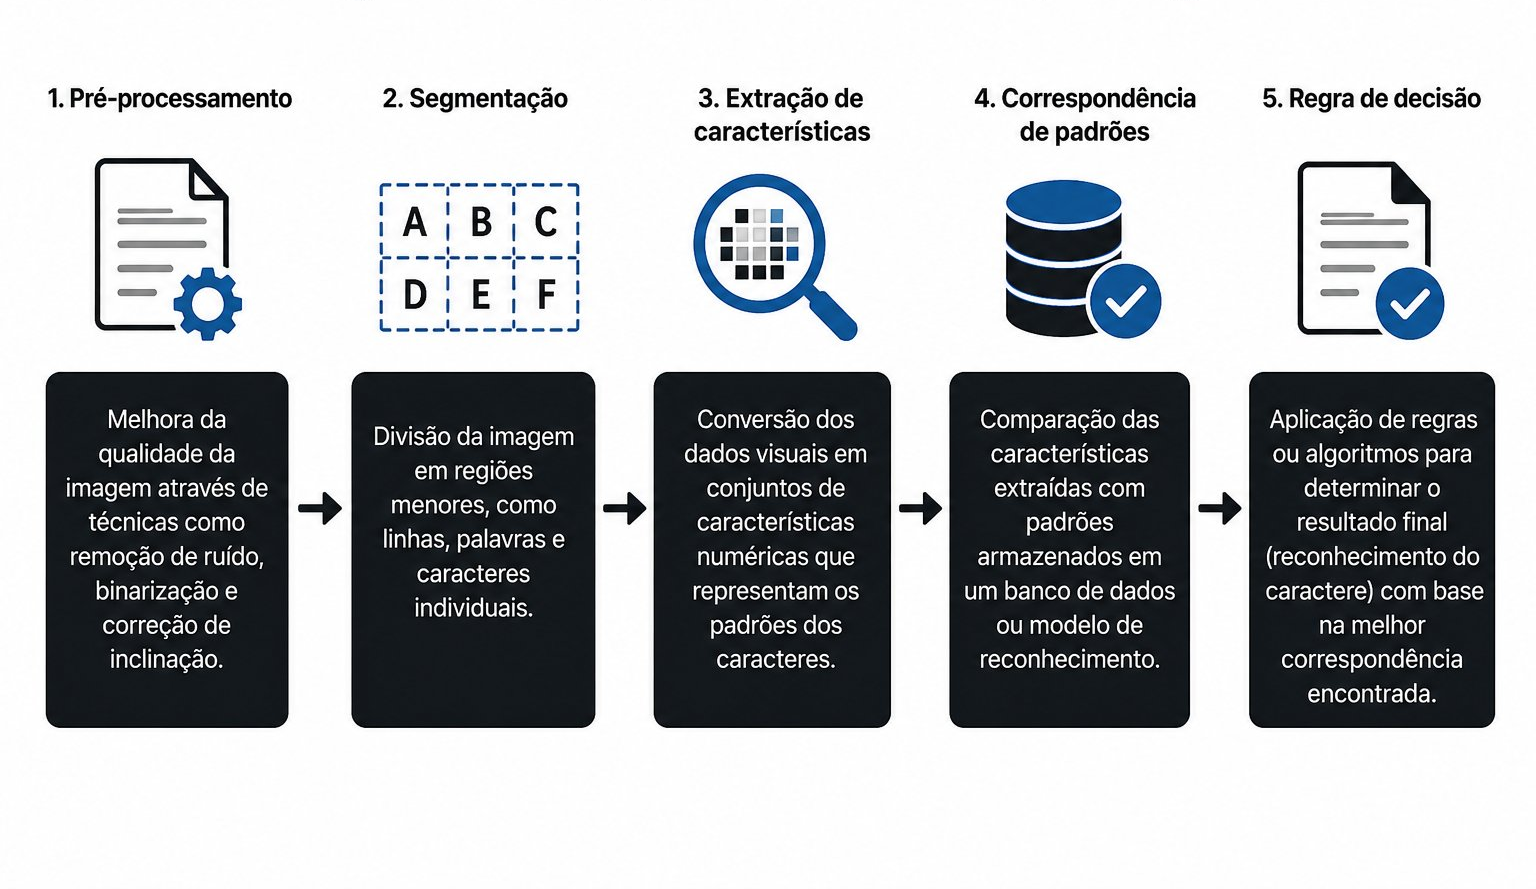
\includegraphics[width=\textwidth]{imagens/ocr-pipeline.png}
    \caption{Diagrama de blocos de um sistema de OCR.}
    \label{fig:ocr_pipeline}
    \fonte{Adaptado de \cite{ocr_diagram}.}
\end{figure}

\subsection{Papel do OCR em Projetos de Digitalização de Acervos}

O OCR tornou-se fundamental para iniciativas de preservação digital de acervos literários
históricos. Bibliotecas, arquivos e instituições de pesquisa utilizam OCR para digitalizar
coleções de obras antigas, transformando volumes frágeis e degradados em formatos
acessíveis e pesquisáveis. Essa transformação não apenas preserva o conteúdo, mas também
democratiza o acesso e viabiliza novas formas de pesquisa e análise que dependem de texto
processável por máquina \cite{EmergenMind2025}.

%---------------------------------------------------------------------
\section{Principais Técnicas de OCR}
\label{sec:tecnicas}
%---------------------------------------------------------------------

A evolução dos sistemas de reconhecimento óptico de caracteres produziu quatro gerações
tecnológicas distintas, cada uma com princípios de funcionamento, pontos fortes e
limitações próprios. Compreender essas diferenças é essencial para justificar a escolha
de ferramentas em contextos específicos, como o de obras literárias antigas em
português. O \textbf{OCR Clássico} opera por segmentação de caracteres e correspondência
com padrões pré-definidos, sendo leve e reprodutível, mas frágil diante de degradação
física. O \textbf{OCR baseado em Aprendizado Profundo} combina redes convolucionais
(CNN) com redes recorrentes (LSTM) para processar linhas de texto, generalizando melhor
do que o clássico, porém ainda dependente de uma segmentação de boa qualidade. Os modelos
\textbf{Transformer} aplicam mecanismos de atenção sobre patches da imagem, capturando
dependências de longo alcance dentro da página, o que os torna mais robustos a variações
tipográficas. Por fim, os \textbf{Modelos de Visão-Linguagem (VLMs)} dispensam qualquer
etapa de segmentação explícita: recebem a imagem completa e geram a transcrição por
geração autorregressiva, aproveitando conhecimento linguístico pré-treinado em larga
escala, ao custo de uma tendência a modernizar grafias históricas. A
Tabela~\ref{tab:tecnicas_ocr} resume essas quatro abordagens segundo seus respectivos princípios de
funcionamento, principais vantagens e limitações mais relevantes para o contexto deste trabalho.

\begin{table}[H]
\centering
\caption{Comparativo das principais técnicas de OCR segundo princípio, vantagens e
limitações.}
\label{tab:tecnicas_ocr}
\renewcommand{\arraystretch}{1.3}
\begin{tabular}{p{2.2cm} p{4cm} p{3.5cm} p{3.5cm}}
\hline
\textbf{Técnica} & \textbf{Princípio} & \textbf{Vantagens} & \textbf{Limitações} \\
\hline
OCR Clássico &
  Segmentação de caracteres + correspondência de padrões &
  Leve, sem GPU, reprodutível &
  Falha com degradação e fontes incomuns \\ \hline
Aprendizado Profundo (CRNN) &
  CNN + LSTM sobre linhas segmentadas &
  Generaliza melhor que o clássico &
  Depende de segmentação de linhas \\ \hline
Transformer (ViT + decoder) &
  Atenção global sobre patches da imagem &
  Captura contexto de longo alcance &
  Sensível a scripts não vistos no treino \\ \hline
VLM &
  Geração autorregressiva sobre imagem completa &
  Sem segmentação; lida com layouts complexos &
  Normaliza ortografia histórica implicitamente \\
\hline
\end{tabular}
\fonte{Elaborado pelo autor.}
\end{table}

\subsection{OCR Clássico}

Os primeiros sistemas de OCR comercialmente viáveis operavam por meio de correspondência
de padrões (\textit{template matching}) e análise de características geométricas dos
glifos. Nessa abordagem, cada caractere é segmentado individualmente da imagem e
comparado a um conjunto de moldes pré-definidos; o caractere cujo molde apresenta maior
similaridade é o reconhecido \cite{Incode2025}. Sistemas mais sofisticados extraíam
características como proporções, ângulos de traços e número de extremidades para treinar
classificadores estatísticos, como máquinas de vetor de suporte (SVM).

A principal limitação dessa abordagem em documentos históricos é a dependência de uma
segmentação precisa: quando a degradação física distorce ou une caracteres adjacentes,
toda a cadeia de reconhecimento é prejudicada. Além disso, fontes e estilos tipográficos
não presentes no conjunto de treinamento resultam em taxas de erro elevadas
\cite{lombardi2020}.

\subsection{OCR Baseado em Aprendizado Profundo}

A partir dos anos 2010, redes neurais convolucionais (CNNs) passaram a substituir os
classificadores tradicionais no núcleo dos sistemas OCR. Em vez de extrair características
manualmente definidas, as CNNs aprendem representações hierárquicas diretamente dos
pixels da imagem durante o treinamento, tornando-se capazes de generalizar para variações
tipográficas e de qualidade que os métodos clássicos não conseguiam tratar
\cite{lombardi2020}.

Uma arquitetura amplamente adotada combina CNNs para extração de características visuais
com redes neurais recorrentes do tipo LSTM (\textit{Long Short-Term Memory}) para
modelagem sequencial do texto, formando o que se denomina
\href{https://arxiv.org/abs/1507.05717}{CRNN} (\textit{Convolutional Recurrent Neural
Network}). Essa combinação permite que o modelo considere o contexto de caracteres
vizinhos ao realizar o reconhecimento, reduzindo ambiguidades. Embora ofereçam desempenho
superior ao OCR clássico em documentos com degradação moderada, esses modelos ainda
dependem de segmentação de linhas de qualidade e podem falhar em tipografias muito
distintas das presentes em seus dados de treinamento \cite{dataunboxed2025}.

\subsection{OCR Baseado em Transformers}

A arquitetura Transformer, introduzida originalmente para processamento de linguagem
natural, foi adaptada para visão computacional com o desenvolvimento do Vision Transformer
(ViT), que divide a imagem em patches e aplica mecanismos de atenção para capturar
dependências globais entre regiões distantes da imagem \cite{huang2021}. No contexto de
OCR, essa capacidade é particularmente relevante: ao contrário das CNNs, que processam a
imagem de forma local e hierárquica, o Transformer pode relacionar diretamente um traço
em uma extremidade da linha com o contexto tipográfico em outra.

Modelos baseados nessa arquitetura combinam um encoder visual do tipo ViT com um decoder
de linguagem em uma estrutura encoder-decoder de ponta a ponta, pré-treinada em larga
escala e refinada para tarefas específicas de reconhecimento. Avaliações recentes mostram
que essa abordagem supera sistemas baseados em CRNN em benchmarks padrão, mas permanece
sensível à qualidade da segmentação de linhas e a scripts não vistos durante o
treinamento, limitação relevante para obras do século XVIII \cite{vesalainen2025}.

\subsection{Modelos de Visão-Linguagem (VLMs)}

A geração mais recente de sistemas de reconhecimento de texto é composta por modelos de
visão-linguagem (\textit{Vision-Language Models}, VLMs), que processam a imagem completa
da página, sem etapa explícita de segmentação de linhas ou caracteres, e geram a
transcrição como saída de um modelo de linguagem generativo. Esses modelos recebem a
imagem diretamente e produzem texto por meio de geração autorregressiva, aproveitando o
conhecimento linguístico acumulado durante o pré-treinamento em bilhões de
tokens \cite{dataunboxed2025}.

Essa abordagem apresenta vantagens significativas em documentos com layouts complexos,
múltiplas colunas e mistura de fontes, onde a ausência de uma etapa de segmentação
elimina uma fonte recorrente de erros. Benchmarks recentes indicam que VLMs alcançam
taxas de similaridade textual até três a quatro vezes superiores às dos métodos clássicos
em documentos complexos \cite{dataunboxed2025}. Contudo, uma limitação crítica
identificada por Vesalainen et al.\ \cite{vesalainen2025} é a tendência desses modelos
de realizar normalização ortográfica implícita: ao transcrever textos históricos, VLMs
frequentemente modernizam grafias arcaicas de forma silenciosa, comportamento
problemático para aplicações que exigem fidelidade diplomática ao original.

%---------------------------------------------------------------------
\clearpage
\section{Ferramentas de OCR Avaliadas}
\label{sec:ferramentas}
%---------------------------------------------------------------------

Esta seção apresenta as ferramentas de reconhecimento automático de texto avaliadas neste
trabalho. A seleção abrange as quatro gerações tecnológicas descritas na
Seção~\ref{sec:tecnicas}: OCR clássico, aprendizado profundo (CRNN), Transformers e
modelos de visão-linguagem. Para cada ferramenta são indicados o modelo de acesso, o
regime de custo e os requisitos de hardware, aspectos relevantes para a replicabilidade
do benchmark.

\subsection{OCR Clássico}

O \href{https://github.com/tesseract-ocr/tesseract}{\textbf{Tesseract~5}}
\cite{smith2019} é um motor OCR de código aberto mantido pelo Google, licenciado sob
Apache~2.0. Originalmente desenvolvido pela Hewlett-Packard nos anos 1980, é o único
representante desta categoria que opera de forma genuinamente clássica na etapa de
segmentação: após extrair regiões de texto, utiliza uma rede LSTM interna apenas para o
reconhecimento de linhas já segmentadas, sem detector neural de texto. Opera inteiramente
em CPU, sem necessidade de GPU, e suporta mais de 100 idiomas incluindo o português.

\subsection{OCR Baseado em Aprendizado Profundo (CRNN)}

O \href{https://github.com/JaidedAI/EasyOCR}{\textbf{EasyOCR}} \cite{easyocr2020} é
uma biblioteca Python de código aberto, licenciada sob Apache~2.0, que implementa uma
arquitetura de dois estágios: detecção com o algoritmo
\href{https://arxiv.org/abs/1904.01941}{CRAFT} (\textit{Character Region Awareness for
Text Detection}) seguida de reconhecimento com uma rede
\href{https://arxiv.org/abs/1507.05717}{CRNN} (CNN +
\href{https://en.wikipedia.org/wiki/Long_short-term_memory}{BiLSTM} +
\href{https://en.wikipedia.org/wiki/Connectionist_temporal_classification}{CTC}).
Suporta mais de 80 idiomas e pode utilizar GPU opcionalmente. Sua interface simplificada
a torna acessível sem configuração extensa.

O \href{https://github.com/PaddlePaddle/PaddleOCR}{\textbf{PaddleOCR}}
\cite{paddleocr2022} é desenvolvido pela Baidu e disponibilizado sob licença Apache~2.0.
Utiliza uma arquitetura de três estágios: detecção, classificação de orientação e
reconhecimento, com modelos baseados em redes convolucionais e recorrentes
pré-treinados para múltiplos idiomas. Suporte a GPU é opcional e o modelo para português
está disponível na distribuição padrão.

O \href{https://github.com/mindee/doctr}{\textbf{DocTR}} (\textit{Document Text
Recognition}) \cite{doctr2021} é uma biblioteca de código aberto da Mindee, licenciada
sob Apache~2.0, que implementa pipelines OCR com suporte a backends TensorFlow e PyTorch.
Combina detectores baseados em \href{https://arxiv.org/abs/1911.08947}{DBNet} ou
\href{https://arxiv.org/abs/1707.03718}{LinkNet} com reconhecedores
\href{https://arxiv.org/abs/1507.05717}{CRNN} ou
\href{https://arxiv.org/abs/1811.00751}{SAR}, sendo projetada para documentos
estruturados com suporte opcional a GPU.

\subsection{Baseado em Transformer}

O \href{https://huggingface.co/microsoft/trocr-base-handwritten}{\textbf{TrOCR}}
\cite{huang2021} é um modelo desenvolvido pela Microsoft, disponível gratuitamente no
\href{https://huggingface.co/microsoft/trocr-base-handwritten}{Hugging Face} sob licença
MIT, que combina um encoder Vision Transformer (ViT) com um decoder de linguagem baseado
em Transformer em uma arquitetura \textit{encoder-decoder} pré-treinada em larga escala.
São avaliadas duas variantes:
\href{https://huggingface.co/microsoft/trocr-base-handwritten}{\texttt{base-handwritten}}
e
\href{https://huggingface.co/microsoft/trocr-large-handwritten}{\texttt{large-handwritten}},
ambas treinadas em dados de texto manuscrito e impresso. O uso de GPU é recomendado para
tempo de inferência aceitável, especialmente na variante \textit{large}.

\subsection{Modelos de Visão-Linguagem (VLMs)}

Os modelos de visão-linguagem avaliados neste trabalho podem ser acessados de duas
formas: execução local, por meio do
\href{https://ollama.com}{\textbf{Ollama}} \cite{ollama2023}, uma plataforma de código
aberto que simplifica o download e a execução de modelos em hardware local, ou via
API, em que o processamento ocorre em servidores remotos mediante pagamento por volume
de páginas ou tokens. Os modelos locais oferecem maior controle sobre os dados e custo
zero por inferência, ao custo de exigirem GPU para tempo de resposta aceitável; os
modelos via API eliminam essa dependência de hardware, mas implicam custo financeiro e
envio das imagens a terceiros.

O \href{https://ai.google.dev/gemma/docs/core}{\textbf{Gemma~4}}
\cite{gemma4_modelcard} é desenvolvido pelo Google DeepMind, lançado em abril de 2026
sob licença Apache~2.0. Disponível em quatro tamanhos (E2B, E4B, 26B e 31B) via Ollama,
combina compreensão visual e geração de texto sem etapa explícita de segmentação.

O \href{https://github.com/deepseek-ai/DeepSeek-VL2}{\textbf{DeepSeek-VL2}}
\cite{wu2024deepseekvl2} é desenvolvido pela DeepSeek e disponível via Ollama. Apresenta
arquitetura de mistura de especialistas (\textit{Mixture of Experts}, MoE), com variantes
de 1,0B, 2,8B e 4,5B de parâmetros ativos, permitindo alto desempenho com menor custo
computacional em relação a modelos densos de tamanho equivalente.

O \href{https://github.com/QwenLM/Qwen2.5-VL}{\textbf{Qwen2.5-VL}} \cite{qwen2025vl}
é desenvolvido pelo Qwen Team da Alibaba Cloud, disponível sob licença Apache~2.0 via
Ollama. Projetado para compreensão de documentos, emprega um Vision Transformer de
resolução dinâmica nativa e se destaca em extração estruturada de formulários, tabelas e
layouts complexos \cite{vesalainen2025}.

O \href{https://www.llamaindex.ai/llamaparse}{\textbf{LlamaParse}}
\cite{llamaparse_pricing} é um serviço da LlamaIndex acessado via API, que utiliza
modelos de linguagem de grande porte para extração e análise de documentos. O plano
gratuito inclui 10.000 créditos mensais e o custo por página varia conforme o modo de
processamento, partindo de 1 crédito por página no modo básico (equivalente a
US\$\,0,00125/página) até modos mais avançados, como o Agentic e o Agentic Plus,
que consomem respectivamente 10 e 45 créditos por página, com custos aproximados de
US\$\,0,0125/página e US\$\,0,05625/página. Neste trabalho, é avaliado em duas
configurações: modo básico (\textit{Cost Effective}) e modo agêntico
(\textit{Agentic}), que diferem no modelo subjacente utilizado e, consequentemente,
na qualidade esperada do reconhecimento.

O \href{https://mistral.ai/news/mistral-ocr}{\textbf{Mistral OCR}} \cite{mistral2025}
é um serviço da Mistral AI acessado via API, cobrado a US\$\,2,00 por mil páginas no
modo padrão e US\$\,1,00 via Batch API. Destaca-se pelo suporte a documentos com layouts
complexos e fórmulas matemáticas.

O \href{https://ai.google.dev/gemini-api/docs/models}{\textbf{Gemini~2.0~Flash}}
\cite{gemini_pricing} é um modelo do Google acessado via API, cobrado a
US\$\,0,10 por milhão de tokens de entrada, com camada gratuita disponível. O Google
anunciou a descontinuação desta versão para junho de 2026; caso necessário, deve ser
substituído pelo Gemini~2.5~Flash.

\subsection{Quadro Comparativo das Ferramentas}

A seleção das ferramentas avaliadas neste trabalho foi orientada por dois critérios
principais: cobertura das quatro gerações tecnológicas descritas na
Seção~\ref{sec:tecnicas} e relevância em benchmarks recentes aplicados a documentos
complexos \cite{dataunboxed2025,vesalainen2025}. Selecionamos para este estudo ao menos
uma ferramenta de cada geração tecnológica, dentre as mais populares e bem avaliadas na
literatura e na Web, para garantir uma avaliação abrangente. Porém, optamos por
selecionar um maior número de ferramentas mais recentes, por serem mais promissoras
para lidar com os desafios do OCR em obras antigas. O \textbf{Tesseract~5} foi incluído por
ser a referência canônica de código aberto, amplamente utilizado como \textit{baseline}
em estudos comparativos. O \textbf{EasyOCR} e o \textbf{PaddleOCR} foram escolhidos por
oferecerem suporte explícito ao português e instalação simplificada, enquanto o
\textbf{DocTR} se destaca por integrar detecção e reconhecimento em um único pipeline
moderno baseado em aprendizado profundo.

Na categoria Transformer, o \textbf{TrOCR} é avaliado em duas variantes
(\texttt{base} e \texttt{large}) por ser o modelo mais citado na literatura de OCR
histórico \cite{huang2021}. Entre os VLMs locais, o \textbf{Gemma~4}, o
\textbf{DeepSeek-VL2} e o \textbf{Qwen2.5-VL} foram selecionados por serem executáveis
sem custo via Ollama e por aparecerem em benchmarks recentes com desempenho competitivo
\cite{vesalainen2025}. Por fim, entre os serviços via API, o \textbf{LlamaParse} (nas
camadas gratuita e premium), o \textbf{Mistral OCR} e o \textbf{Gemini~2.0~Flash} foram
incluídos para cobrir o espectro de soluções comerciais com diferentes relações
custo-desempenho, permitindo comparação direta com as alternativas locais.

A Tabela~\ref{tab:ferramentas_fund} apresenta uma visão consolidada de todas as
ferramentas, indicando para cada uma: a categoria tecnológica, a licença de uso, a forma
de acesso (local ou API), o regime de custo e a necessidade de GPU.

\begin{table}[H]
\centering
\caption{Ferramentas de OCR avaliadas: categoria, licença, forma de acesso, custo e
requisito de GPU.}
\label{tab:ferramentas_fund}
\renewcommand{\arraystretch}{1.3}
\begin{tabular}{p{2.3cm} p{2.8cm} p{2cm} p{1.2cm} p{1.8cm} p{2cm}}
\hline
\textbf{Ferramenta} & \textbf{Categoria} & \textbf{Licença} & \textbf{Acesso}
  & \textbf{Custo} & \textbf{GPU} \\
\hline
\href{https://github.com/tesseract-ocr/tesseract}{Tesseract 5}
  & OCR Clássico         & Apache 2.0   & Local & Gratuito  & Não \\
\hline
\href{https://github.com/JaidedAI/EasyOCR}{EasyOCR}
  & Deep Learning (CRNN) & Apache 2.0   & Local & Gratuito  & Opcional \\
\href{https://github.com/PaddlePaddle/PaddleOCR}{PaddleOCR}
  & Deep Learning (CRNN) & Apache 2.0   & Local & Gratuito  & Opcional \\
\href{https://github.com/mindee/doctr}{DocTR}
  & Deep Learning (CRNN) & Apache 2.0   & Local & Gratuito  & Opcional \\
\hline
\href{https://huggingface.co/microsoft/trocr-base-handwritten}{TrOCR \texttt{base}}
  & Transformer          & MIT          & Local & Gratuito  & Recomenda \\
\href{https://huggingface.co/microsoft/trocr-large-handwritten}{TrOCR \texttt{large}}
  & Transformer          & MIT          & Local & Gratuito  & Recomenda \\
\hline
\href{https://ai.google.dev/gemma/docs/core}{Gemma 4 (Ollama)}
  & VLM local            & Apache 2.0   & Local & Gratuito  & Recomenda \\
\href{https://github.com/deepseek-ai/DeepSeek-VL2}{DeepSeek-VL2 (Ollama)}
  & VLM local            & Aberta$^{a}$ & Local & Gratuito  & Recomenda \\
\href{https://github.com/QwenLM/Qwen2.5-VL}{Qwen2.5-VL (Ollama)}
  & VLM local            & Apache 2.0   & Local & Gratuito  & Recomenda \\
\hline
\href{https://www.llamaindex.ai/llamaparse}{LlamaParse Basic}
  & VLM via API          & Proprietária & API   & Pago$^{b}$ & Não \\
\href{https://www.llamaindex.ai/llamaparse}{LlamaParse Agentic}
  & VLM via API          & Proprietária & API   & Pago$^{b}$ & Não \\
\href{https://mistral.ai/news/mistral-ocr}{Mistral OCR}
  & VLM via API          & Proprietária & API   & Pago$^{c}$ & Não \\
\href{https://ai.google.dev/gemini-api/docs/models}{Gemini 2.0 Flash}
  & VLM via API          & Proprietária & API   & Pago$^{d}$ & Não \\
\hline
\multicolumn{6}{p{14.5cm}}{%
  \footnotesize
  $^{a}$~DeepSeek-VL2: licença DeepSeek Model License (uso comercial permitido com
  restrições).
  $^{b}$~LlamaParse opera por créditos (10.000 créditos/mês no plano gratuito):
  modo Basic custa 1 crédito/página (US\$\,0,00125/pág.); modo Agentic custa
  10 créditos/página (US\$\,0,0125/pág.) \cite{llamaparse_pricing}.
  $^{c}$~Mistral OCR: US\$\,2,00/1.000 páginas (padrão) ou US\$\,1,00/1.000 páginas
  (Batch API) \cite{mistral2025}.
  $^{d}$~Gemini 2.0 Flash: US\$\,0,10/milhão de tokens de entrada
  \cite{gemini_pricing}; descontinuação prevista para jun./2026.
} \\
\end{tabular}
\fonte{Elaborado pelo autor.}
\end{table}

%---------------------------------------------------------------------
\section{Métricas de Avaliação de Soluções para OCR}
%---------------------------------------------------------------------

A qualidade do reconhecimento automático de texto é mensurada por meio de métricas que
comparam a saída do sistema com um texto de referência produzido manualmente, denominado
\textit{regra ouro} (\textit{ground truth}). As métricas mais consolidadas na literatura
de OCR são o Word Error Rate (WER) e o Character Error Rate (CER), que quantificam,
respectivamente, os erros ao nível da palavra e do caractere. Esta seção apresenta essas
métricas, sua complementariedade e os valores típicos esperados para diferentes tipos de
documento.

\subsection{Word Error Rate (WER)}

O Word Error Rate (WER) avalia a precisão do OCR ao nível da palavra, medindo a
proporção de palavras reconhecidas incorretamente em relação ao total de palavras no
texto de referência. A fórmula é:

\[
\text{WER} = \frac{S + D + I}{N} \times 100\%
\]

onde:
\begin{itemize}
    \item $S$ = número de substituições (uma palavra foi reconhecida como uma palavra
    diferente);
    \item $D$ = número de deleções (uma palavra foi omitida);
    \item $I$ = número de inserções (uma palavra extra foi adicionada);
    \item $N$ = número total de palavras na referência.
\end{itemize}

WER é apropriada para OCR porque mede erros no nível de unidades semânticas
(palavras) \cite{ScienceDirect2025}. Um erro em um único caractere que resulte em uma
palavra totalmente diferente é contado como um erro de palavra. Para publicações limpas
e bem impressas, alvos típicos de WER são abaixo de 5\%, enquanto para obras históricas
podem esperar-se valores bem maiores \cite{DocuClipper2025}.

\subsection{Character Error Rate (CER)}

O Character Error Rate (CER) mede a precisão ao nível individual de caracteres,
oferecendo uma visão mais granular dos erros. A fórmula é idêntica à de WER, mas
aplicada a caracteres:

\[
\text{CER} = \frac{S + D + I}{N} \times 100\%
\]

onde agora $N$ é o número total de caracteres na referência.

CER é particularmente efetiva quando pequenos erros têm consequências significativas,
como em linguagens tônicas ou baseadas em script, onde uma alteração de um único
caractere pode mudar completamente o significado \cite{Galileo2025}. Em português
histórico, onde diacríticos distinguem palavras diferentes, CER é uma métrica
especialmente importante. Adicionalmente, CER é mais apropriada para linguagens sem
limites claros de palavras \cite{Advocating2025}.

\subsection{Complementariedade entre CER e WER}

CER geralmente resulta em valores menores que WER porque um erro em um único caractere
afeta apenas um caractere na métrica CER, mas pode afetar uma ou mais palavras na métrica
WER. Por exemplo, uma taxa de CER de 5\% pode corresponder a uma WER de 25\% ou superior,
dependendo da estrutura da língua \cite{WaterCrawl2025}.

Para avaliação abrangente de sistemas OCR, ambas as métricas devem ser reportadas, pois
capturam diferentes aspectos da qualidade: CER fornece informações sobre precisão em nível
fino, enquanto WER mede o impacto prático dos erros na legibilidade de
palavras \cite{TowardsDataScience2025}.

\subsection{Acurácia em Diferentes Contextos}

É importante notar que a precisão do OCR varia significativamente conforme o tipo de
material. Texto impresso limpo e bem digitalizado pode alcançar precisão de 95--99\% com
mecanismos modernos, enquanto obras históricas, layouts complexos e imagens de baixa
qualidade tipicamente ficam no intervalo de 50--90\% de acurácia \cite{PictureText2025}.
Essa variação reflete a dificuldade aumentada de processar publicações que se desviam do
padrão de texto moderno bem-definido.

\subsection{Validação Qualitativa e Inspeção Manual}

Além de métricas quantitativas como CER e WER, a validação qualitativa por meio de
inspeção visual dos resultados é essencial. Essa análise permite a categorização dos
erros em duas categorias principais:

\begin{itemize}
    \item \textit{Erros Sistemáticos}: ocorrem de forma recorrente sob determinadas
    condições, como a confusão consistente entre caracteres visualmente similares (por
    exemplo, ``l'' e ``I'') em uma mesma fonte.

    \item \textit{Erros Isolados}: manifestam-se de maneira esporádica, sendo geralmente
    atribuídos a ruído ou a características específicas de páginas individuais.
\end{itemize}

Erros sistemáticos sugerem limitações fundamentais do modelo que poderiam ser corrigidas
por meio de retreinamento ou pós-processamento específico, enquanto erros isolados podem
ser mais fáceis de tratar mediante limpeza de dados ou ajustes localizados. A inspeção
manual também permite entender o contexto dos erros: um caractere pode ser confundido com
outro com maior frequência em certos tipos de layout, resoluções específicas de
digitalização, ou estilos tipográficos \cite{EmergenMind2025}.

%=====================================================================
% CAPÍTULO 3: TRABALHOS RELACIONADOS
%=====================================================================
\chapter{Trabalhos Relacionados}

Este capítulo apresenta trabalhos relacionados ao reconhecimento óptico de caracteres em
documentos históricos e obras literárias. A Seção~\ref{sec:metodologia_revisao} descreve
o processo de busca e seleção bibliográfica adotado. Em seguida, os trabalhos são
organizados em três eixos temáticos: a Seção~\ref{sec:ocr_historico} discute pesquisas
voltadas ao OCR em documentos históricos e degradados de forma geral, abordando técnicas
de pré-processamento, arquiteturas de reconhecimento e os principais desafios do domínio.
A Seção~\ref{sec:ocr_portugues} focaliza especificamente o estado da arte em OCR para a
língua portuguesa, evidenciando a escassez de recursos e modelos dedicados ao idioma.
Por fim, a Seção~\ref{sec:ocr_historico_pt} restringe o escopo à interseção entre OCR e
documentos históricos escritos em português, situando o presente trabalho em relação às
iniciativas mais próximas do problema aqui tratado.

\section{Processo de Busca e Seleção Bibliográfica}
\label{sec:metodologia_revisao}

A revisão bibliográfica apresentada neste capítulo, assim como parte da fundamentação
teórica do Capítulo~2, foi conduzida por meio de buscas exploratórias em fontes
acadêmicas. As buscas
cobriram conteúdo indexado em bases como Google Scholar, IEEE Xplore e ACM Digital, complementadas pontualmente por
documentação técnica oficial de ferramentas (páginas de projeto, repositórios de código
e documentação de API) para a obtenção de especificações factuais sobre produtos
específicos, sem valor de embasamento teórico.

As buscas foram realizadas tanto em português quanto em inglês, combinando termos
relacionados à tecnologia de OCR, ao domínio de aplicação e ao idioma-alvo. Entre as
palavras-chave utilizadas estão: "OCR ferramentas comparação", "\textit{OCR
documentos históricos português}", "\textit{reconhecimento óptico de caracteres avaliação}",
\textit{"OCR manuscritos históricos português}", "\textit{historical OCR benchmark}",
\textit{"vision-language model OCR historical documents}", "\textit{Handwritten Text
Recognition historical documents}", \textit{"OCR post-correction Portuguese};",\textit{"large
language model OCR correction}", "\textit{Character Error Rate" ,"Word Error Rate" e "OCR
evaluation}". Buscas adicionais e mais específicas foram realizadas a partir dos nomes de
ferramentas e modelos identificados nas etapas anteriores (ex: \textit{"Tesseract
EasyOCR PaddleOCR TrOCR comparison"}), bem como a partir de autores e termos citados por
trabalhos já localizados por outros meios.

O período priorizado foi de 2018 a 2026, com ênfase em publicações a partir de 2023,
dado o ritmo acelerado de evolução de arquiteturas baseadas em Transformers e em modelos
de visão-linguagem aplicados a OCR. Buscas amplas iniciais, voltadas ao mapeamento geral do
estado da arte em OCR, foram seguidas de buscas direcionadas a lacunas identificadas
(como OCR aplicado especificamente ao português e a documentos históricos), e
complementadas por \textit{snowballing} a partir das referências dos trabalhos mais
relevantes encontrados, como Vesalainen et al.\ \cite{vesalainen2025}.

Foram excluídos trabalhos
sem relação direta com OCR, ou digitalização de texto, bem como conteúdo puramente
promocional ou de caráter comercial sem embasamento metodológico, este último mantido
apenas como fonte factual para especificações técnicas de ferramentas (Seção~2.4), e não
como referência de embasamento teórico. Esse processo resultou nos sete trabalhos
diretamente relacionados discutidos nas seções seguintes deste capítulo, sintetizados na
Tabela~\ref{tab:trabalhos_relacionados}, complementados pelas referências de
fundamentação teórica e técnica apresentadas no Capítulo~2.

\section{OCR para Documentos Históricos e Degradados}
\label{sec:ocr_historico}

A aplicação de OCR a obras literárias históricas constitui um subcampo com desafios
próprios e crescente atenção da comunidade de visão computacional. Diferentemente de
publicações modernas com tipografia padronizada e alta qualidade de impressão, as obras
históricas apresentam condições que sistematicamente prejudicam os motores de
reconhecimento, seja por degradação do suporte físico, tinta desbotada ou infiltrada no
verso da página (\textit{bleed-through}), iluminação desigual nas digitalizações ou por
variações tipográficas da época e ortografia não padronizada \cite{lombardi2020}.

O pré-processamento das imagens constitui a primeira linha de defesa contra essas
dificuldades. A binarização (conversão da imagem colorida ou em tons de cinza para
preto e branco) é uma etapa fundamental, pois separa o conteúdo textual de fatores de
ruído como manchas, fundos não uniformes e entintamento irregular \cite{lombardi2020}.
Abordagens baseadas em aprendizado profundo, como redes convolucionais e arquiteturas do
tipo U-Net, têm superado os métodos tradicionais de limiarização nessa tarefa,
especialmente em documentos com alto grau de degradação \cite{anvari2021}. Apesar desses
avanços, sistemas OCR frequentemente falham no reconhecimento de padrões de caracteres
quando a degradação é severa, e a escassez de dados anotados para treinamento agrava
essas dificuldades \cite{lombardi2020}.

Com a introdução de arquiteturas baseadas em Transformers, o estado da arte no
reconhecimento de obras literárias históricas avançou significativamente. O modelo
TrOCR \cite{huang2021}, que combina um encoder visual do tipo Vision Transformer (ViT)
com um decoder de linguagem, apresentou desempenho superior aos métodos anteriores em
tarefas de reconhecimento de texto impresso e manuscrito, tornando-se uma referência
importante na área. No entanto, avaliações recentes indicam que modelos baseados em
Transformers ainda enfrentam limitações relevantes no contexto histórico, pois são
sensíveis à qualidade da segmentação de linhas, a fontes e scripts não vistos durante o
treinamento, e à degradação específica de materiais antigos \cite{vesalainen2025}.

Um aspecto crítico identificado na literatura recente diz respeito ao comportamento dos
modelos de linguagem de grande porte (LLMs) quando aplicados à transcrição histórica.
Embora modelos de visão-linguagem (\textit{Vision-Language Models}, VLMs) como o Qwen
apresentem menores taxas de CER e WER em comparação com abordagens OCR dedicadas, eles
tendem a realizar normalização ortográfica implícita, modernizando grafias históricas de
forma silenciosa \cite{vesalainen2025}. Esse comportamento pode ser problemático para
aplicações acadêmicas que requerem fidelidade diplomática ao texto original, como é o
caso deste trabalho. Modelos OCR dedicados preservam a fidelidade ortográfica com maior
consistência, mas são mais suscetíveis à propagação de erros em cascata.

\section{OCR em Português}
\label{sec:ocr_portugues}

Apesar do português ser uma das línguas com maior número de falantes no mundo, a
pesquisa em OCR voltada especificamente a esse idioma permanece consideravelmente menos
desenvolvida do que para o inglês ou outras línguas europeias de maior recurso
computacional. Essa lacuna é reconhecida pela própria comunidade científica; Santos
et al.\ \cite{santos2023} afirmam explicitamente que o OCR em português permanece
largamente inexplorado, mesmo considerando a expressiva base de falantes do idioma.

Do ponto de vista técnico, o português apresenta características que aumentam a
dificuldade do reconhecimento automático, como o uso extensivo de diacríticos (til,
agudo, circunflexo, grave e cedilha), a alta frequência de vogais acentuadas e, no caso
de textos históricos do século XIX, a presença de ortografia pré-reformas, com grafias
arcaicas e variações não padronizadas que diferem substancialmente das formas modernas.
Sistemas como o Tesseract, quando configurados sem o modelo de linguagem específico para
português, tendem a omitir ou substituir incorretamente esses diacríticos, gerando erros
que, embora pareçam menores no nível do caractere, produzem palavras semanticamente
distintas ou inexistentes no nível da palavra \cite{smith2019}.

No contexto da pós-correção de OCR em português, estudos recentes demonstram que modelos
de linguagem de grande porte baseados em Transformers podem reduzir substancialmente as
taxas de erro residual. Fritzen \cite{fritzen2025} avaliou a aplicação de LLMs como
Gemma~3 para correção pós-OCR no ESTER-Pt, demonstrando que tais modelos conseguem
reduzir o CER do estado da arte em português de 5,12 para 1,69, uma melhoria de
aproximadamente 67\%. Esses resultados evidenciam tanto o potencial dos modelos de
linguagem para o idioma quanto a persistência de erros que métodos puramente baseados em
OCR não conseguem eliminar sem auxílio de contexto linguístico.

A escassez de modelos OCR treinados especificamente em corpora históricos em português,
diferentemente do que existe para o alemão, o inglês ou o latim, representa um desafio
direto para iniciativas como a do NUPILL. Na ausência de modelos para o domínio, a
avaliação comparativa de abordagens disponíveis, combinada com análise qualitativa dos
padrões de erro, torna-se o caminho metodologicamente mais rigoroso para identificar a
solução mais adequada, que é justamente o que este trabalho propõe.

\section{OCR em Documentos Históricos em Língua Portuguesa}
\label{sec:ocr_historico_pt}

A interseção entre OCR e documentos históricos escritos em português constitui um campo
ainda escasso, mas com contribuições recentes que permitem situar o presente trabalho em
relação ao estado da arte.

Rosa et al.\ \cite{rosa2025} conduziram um estudo de caso envolvendo as ferramentas
Google Vision, Docsumo e Transkribus aplicadas à transcrição de manuscritos históricos
brasileiros dos séculos XVIII e XIX, escritos em língua portuguesa. Os resultados
demonstraram que, embora essas ferramentas apresentem desempenho satisfatório em
documentos impressos contemporâneos, ainda enfrentam limitações significativas na
transcrição de manuscritos históricos. Entre os principais desafios identificados estão
a complexidade da caligrafia, a degradação física dos documentos e as variações
linguísticas decorrentes da evolução da língua ao longo do tempo. O estudo conclui que
o avanço contínuo das tecnologias de OCR, aliado ao uso de técnicas de inteligência
artificial, é essencial para atender às especificidades da escrita manual histórica em
português.

No âmbito dos manuscritos históricos portugueses, Aguilar e Jolivet \cite{aguilar2024}
apresentaram um experimento de transcrição automática de manuscritos da Inquisição
portuguesa do século XVI utilizando duas ferramentas de HTR (\textit{Handwritten Text
Recognition}): o \href{https://www.transkribus.org}{Transkribus}, desenvolvido pela
ReadCoop, e o Lapelinc Transcriptor, desenvolvido pelo Laboratório de Linguística de
Corpus da Universidade Estadual do Sudoeste da Bahia. O experimento concentrou-se na
modelagem da escrita de um único copista e na comparação das transcrições automáticas
com transcrições diplomáticas produzidas manualmente, sob perspectiva paleográfica. Os
resultados revelaram que a expertise paleográfica desempenha papel fundamental não apenas
na interpretação dos resultados, mas também na melhoria do desempenho dos modelos HTR,
evidenciando a necessidade de colaboração entre especialistas em humanidades e
desenvolvedores de tecnologia.

Em escala maior, o projeto TraPrInq \cite{baudry2023} aplicou o Transkribus à transcrição
de aproximadamente 6.000 documentos digitalizados dos processos da Inquisição portuguesa.
Ao longo de nove sessões de treinamento realizadas entre junho de 2022 e julho de 2023,
o modelo de reconhecimento de texto em português foi progressivamente refinado a ponto
de, a partir da quarta sessão, a transcrição manual poder ser gradualmente substituída
pela correção das saídas automáticas do motor. O projeto foi apresentado na conferência
Humanidades Digitais e Estudos Inquisitoriais em 2023, e seus resultados demonstram que,
com volume suficiente de anotação e iteração de treinamento, é possível atingir qualidade
prática em documentos históricos em português, mesmo para caligrafia do século XVII.

Em conjunto, esses trabalhos evidenciam que o reconhecimento automático de texto em
documentos históricos em língua portuguesa tem sido abordado quase exclusivamente sob a
perspectiva de manuscritos. O presente trabalho se diferencia ao focar em obras literárias
\textit{impressas} de diferentes períodos, avaliando sistematicamente ferramentas de OCR
modernas, incluindo VLMs, sobre um corpus estratificado por dificuldade, contribuindo
para preencher essa lacuna na literatura.

\section{Síntese Comparativa dos Trabalhos Relacionados}
\label{sec:sintese_relacionados}

A Tabela~\ref{tab:trabalhos_relacionados} sintetiza os trabalhos revisados neste
capítulo segundo cinco dimensões: tipo de documento, idioma do corpus, ferramentas
avaliadas, métricas reportadas e principal contribuição. A linha final destaca como
o presente trabalho se posiciona em relação ao estado da arte.

\begin{table}[H]
\centering
\caption{Síntese comparativa dos trabalhos relacionados em OCR para documentos
históricos.}
\label{tab:trabalhos_relacionados}
\renewcommand{\arraystretch}{1.4}
\begin{tabular}{p{2.5cm} p{2.2cm} p{2cm} p{2.8cm} p{2cm} p{3.0cm}}
\hline
\textbf{Trabalho} &
\textbf{Tipo} &
\textbf{Idioma} &
\textbf{Ferramentas} &
\textbf{Métricas} &
\textbf{Contribuição} \\
\hline
Vesalainen et al.\ \cite{vesalainen2025} &
  Impresso histórico & Finlandês &
  TrOCR, Qwen2.5-VL & CER, WER &
  Padrões de erro e normalização ortográfica implícita por VLMs \\
\hline
Data Unboxed \cite{dataunboxed2025} &
  Impresso moderno & Inglês &
  Tesseract, EasyOCR, VLMs & Sim. textual &
  Benchmark OCR clássico vs.VLMs \\
\hline
Santos et al.\ \cite{santos2023} &
  Impresso moderno & Português &
    - & CER &
  benchmark OCR para português \\
\hline
Fritzen \cite{fritzen2025} &
  Impresso moderno & Português &
  Gemma~3 (pós-OCR) & CER &
  CER reduzido de 5,12 para 1,69 via LLM \\
\hline
Rosa et al.\ \cite{rosa2025} &
  Manuscrito histórico & Português &
  Google Vision, Docsumo, Transkribus & Qualitativa &
  Manuscritos brasileiros sécs.\ XVIII--XIX \\
\hline
Aguilar e Jolivet \cite{aguilar2024} &
  Manuscrito histórico & Português &
  Transkribus, Lapelinc & CER &
  HTR inquisitorial; expertise paleográfica \\
\hline
Baudry \cite{baudry2023} &
  Manuscrito histórico & Português &
  Transkribus & Qualitativa &
  6.000 docs.\ inquisitoriais; treino iterativo \\
\hline
\textbf{Este trabalho} &
  \textbf{Impresso histórico} & \textbf{Português} &
  \textbf{13 ferramentas (clássico, CRNN, Transformer, VLM)} &
  \textbf{CER, WER} &
  \textbf{Benchmark com corpus estratificado} \\
\hline
\end{tabular}
\fonte{Elaborado pelo autor.}
\end{table}
A análise evidencia duas lacunas que o presente trabalho busca preencher. Primeiro,
os estudos em língua portuguesa concentram-se em manuscritos históricos
\cite{rosa2025,aguilar2024,baudry2023} ou em texto impresso contemporâneo
\cite{santos2023,fritzen2025}, sem avaliar obras literárias \textit{impressas}
de períodos anteriores ao século XX. Segundo, nenhum trabalho revisado combina, em um
único benchmark para o português histórico, ferramentas das quatro gerações tecnológicas
(OCR clássico, CRNN, Transformer e VLMs) com corpus estratificado por dificuldade
e métricas padronizadas de CER e WER.

%=====================================================================
% CAPÍTULO 4: CONSTRUÇÃO DA REGRA OURO
%=====================================================================
\chapter{Construção da Regra Ouro}

A avaliação objetiva de sistemas de reconhecimento óptico de caracteres requer a
existência de um conjunto de referência, denominado \textit{regra ouro}, composto por
transcrições manuais fiéis ao conteúdo das imagens originais. Sem esse referencial, não
é possível calcular métricas como WER e CER de forma confiável, pois não há texto correto
com o qual comparar as saídas dos modelos. Este capítulo descreve como essa regra ouro
foi constituída: a origem do corpus, os critérios de seleção das obras e das páginas, a
classificação de dificuldade adotada, o processo de transcrição manual e o procedimento
de validação.

\section{Origem do Corpus}

As obras que compõem o corpus deste trabalho pertencem ao acervo digital do Núcleo de
Pesquisas em Informática, Literatura e Linguística (NUPILL), da Universidade Federal de
Santa Catarina. O NUPILL mantém uma coleção de textos literários históricos digitalizados,
com foco em obras da literatura brasileira e portuguesa, e tem como missão a preservação
e o estudo do patrimônio literário por meio de ferramentas computacionais.

A seleção das obras foi realizada em colaboração com o Prof.\ Dr.\ Alckmar Luiz dos
Santos, pesquisador do NUPILL, que indicou volumes representativos do acervo cujas
digitalizações apresentam características adequadas para um estudo de benchmark de OCR:
imagens em formato PDF com camada de imagem, digitalizadas a 300 DPI pelo software ABBYY
FineReader, cobrindo um espectro variado de condições tipográficas e de degradação física.

\section{Critérios de Seleção das Obras}

A seleção priorizou obras que, em conjunto, cobrissem diferentes graus de dificuldade
para o reconhecimento automático de texto. Três critérios principais orientaram a escolha:

\begin{enumerate}
    \item \textbf{Variação tipográfica}: presença de tipos serifados modernos, itálicos
    densos e tipografia do século XVIII com caracteres arcaicos, de modo a expor os
    modelos a diferentes estilos gráficos.

    \item \textbf{Grau de degradação física}: desde páginas com baixo ruído e bordas
    limpas até páginas com manchas sobre o corpo do texto, contraste reduzido e bordas
    deterioradas.

    \item \textbf{Complexidade ortográfica}: ortografia da virada do século XX, com
    diacríticos e grafias em desuso, até ortografia pré-moderna com caracteres fundidos
    e ausência de espaçamento uniforme.
\end{enumerate}

Com base nesses critérios, foram selecionadas cinco obras do acervo NUPILL, descritas na
Tabela~\ref{tab:obras_corpus}.

\begin{table}[H]
\centering
\caption{Obras selecionadas para composição do corpus de avaliação.}
\label{tab:obras_corpus}
\renewcommand{\arraystretch}{1.3}
\begin{tabular}{p{4.5cm} p{3.5cm} r r p{3.2cm}}
\hline \hline
\textbf{Obra} & \textbf{Autor} & \textbf{Ano} & \textbf{Págs.} & \textbf{Tipografia} \\
\hline \hline
\textit{Heloíza}
  & J. Mariano de Oliveira & c.\ 1910 & 144  & Séc.\ XX, serifada \\ \hline
\textit{Culto à Mulher} (vol.\,1)
  & J. Mariano de Oliveira & c.\ 1920 & 254  & Séc.\ XX, itálica \\ \hline
\textit{Culto à Mulher} (vol.\,2)
  & J. Mariano de Oliveira & 1934     & 219  & Séc.\ XX, monoespaçada \\ \hline
\textit{A Amante Militar}
  & Anônimo                & c.\ 1790 & 110  & Séc.\ XVIII, arcaica \\ \hline
\textit{O Feliz Independente}
  & Pe.\ T.\ de Melo       & c.\ 1779 & 1043 & Séc.\ XVIII, arcaica \\
\hline \hline
\end{tabular}
\fonte{Elaborado pelo autor.}
\end{table}

\section{Classificação de Dificuldade}

Para estruturar a avaliação de forma estratificada, as páginas selecionadas foram
classificadas em três níveis de dificuldade: fácil, médio e difícil. Essa classificação
baseia-se em três eixos observáveis diretamente nas imagens digitalizadas: qualidade
tipográfica, grau de degradação física e complexidade ortográfica.

\subsection{Páginas Fáceis}

Páginas classificadas como fáceis apresentam tipografia serifada regular, com espaçamento
uniforme entre palavras e linhas, característica de impressões do início do século XX. A
degradação física é mínima: eventuais manchas ou ruídos restringem-se às bordas da
página, sem afetar o corpo do texto. A ortografia, embora reflita grafias em desuso (como
\textit{caza}, \textit{pozitivista} e \textit{si} no lugar de \textit{se}), não apresenta
caracteres arcaicos ou ambíguos. Essas condições permitem que modelos OCR convencionais
operem próximo ao seu desempenho nominal.

As páginas de \textit{Heloíza} são representativas dessa classe. A
Figura~\ref{fig:pagina_facil} ilustra um exemplo típico.

\begin{figure}[H]
    \centering
    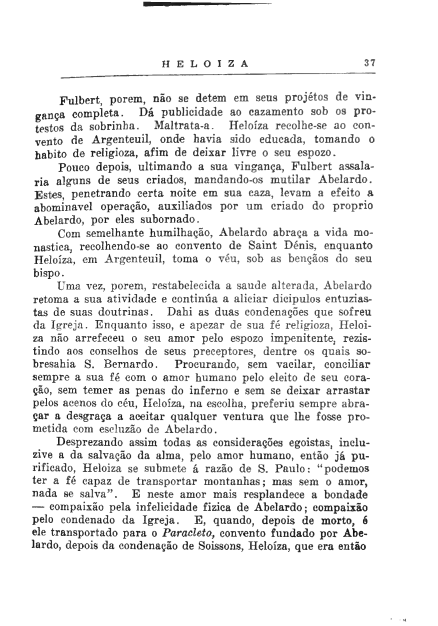
\includegraphics[width=0.75\textwidth]{imagens/heloiza_p040.png}
    \caption{Exemplo de página fácil: \textit{Heloíza}, p.\ 40. Tipografia serifada,
    baixa degradação.}
    \label{fig:pagina_facil}
    \fonte{NUPILL/UFSC.}
\end{figure}

\subsection{Páginas de Dificuldade Média}

Páginas classificadas com dificuldade média caracterizam-se pela presença de múltiplos
estilos tipográficos em uma mesma página, combinando trechos em fonte redonda, itálica e
negrito de forma intercalada. Além disso, observa-se um nível moderado de degradação
física, que pode comprometer parcialmente a legibilidade do corpo textual. Elementos de
layout não convencionais, como poemas com recuos irregulares, notas de rodapé e tabelas
de datas, também contribuem para elevar a complexidade do processo de reconhecimento
óptico de caracteres. Embora a ortografia apresente características semelhantes às
encontradas em páginas de baixa dificuldade, a diversidade tipográfica introduz
ambiguidades adicionais, dificultando o desempenho dos modelos de OCR.

Os volumes de \textit{Culto à Mulher} são representativos dessa classe. A
Figura~\ref{fig:pagina_media} ilustra um exemplo.

\begin{figure}[H]
    \centering
    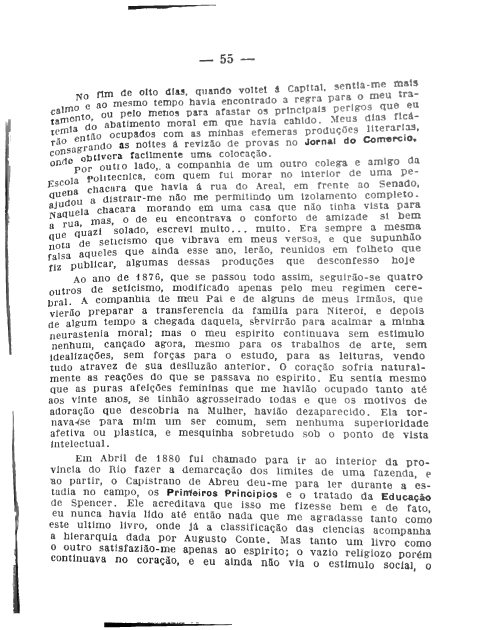
\includegraphics[width=0.75\textwidth]{imagens/culto_p055.png}
    \caption{Exemplo de página de dificuldade média: \textit{Culto à Mulher} vol.\,1,
    p.\ 55. Itálico denso, ruído nas bordas.}
    \label{fig:pagina_media}
    \fonte{NUPILL/UFSC.}
\end{figure}

\subsection{Páginas Difíceis}

Páginas classificadas como difíceis apresentam uma combinação de fatores que tornam o
reconhecimento óptico de caracteres significativamente mais complexo. Destaca-se a
tipografia compacta típica do século XVIII, marcada pela fusão de caracteres, ausência de
espaçamento padronizado e pouca distinção visual entre determinados glifos. Soma-se a
isso o elevado nível de degradação física dos documentos, incluindo manchas sobre o corpo
do texto, bordas escurecidas e redução do contraste, fatores que comprometem diretamente
a legibilidade. Além dos desafios visuais, a presença de ortografia pré-moderna, com
grafias como \textit{hum}, \textit{aquella} e o uso do $s$ longo, impõe dificuldades
adicionais aos modelos de OCR, geralmente treinados com base em textos contemporâneos e
padrões ortográficos modernos.

As páginas de \textit{A Amante Militar} são representativas dessa classe. A
Figura~\ref{fig:pagina_dificil} ilustra um exemplo.

\begin{figure}[H]
    \centering
    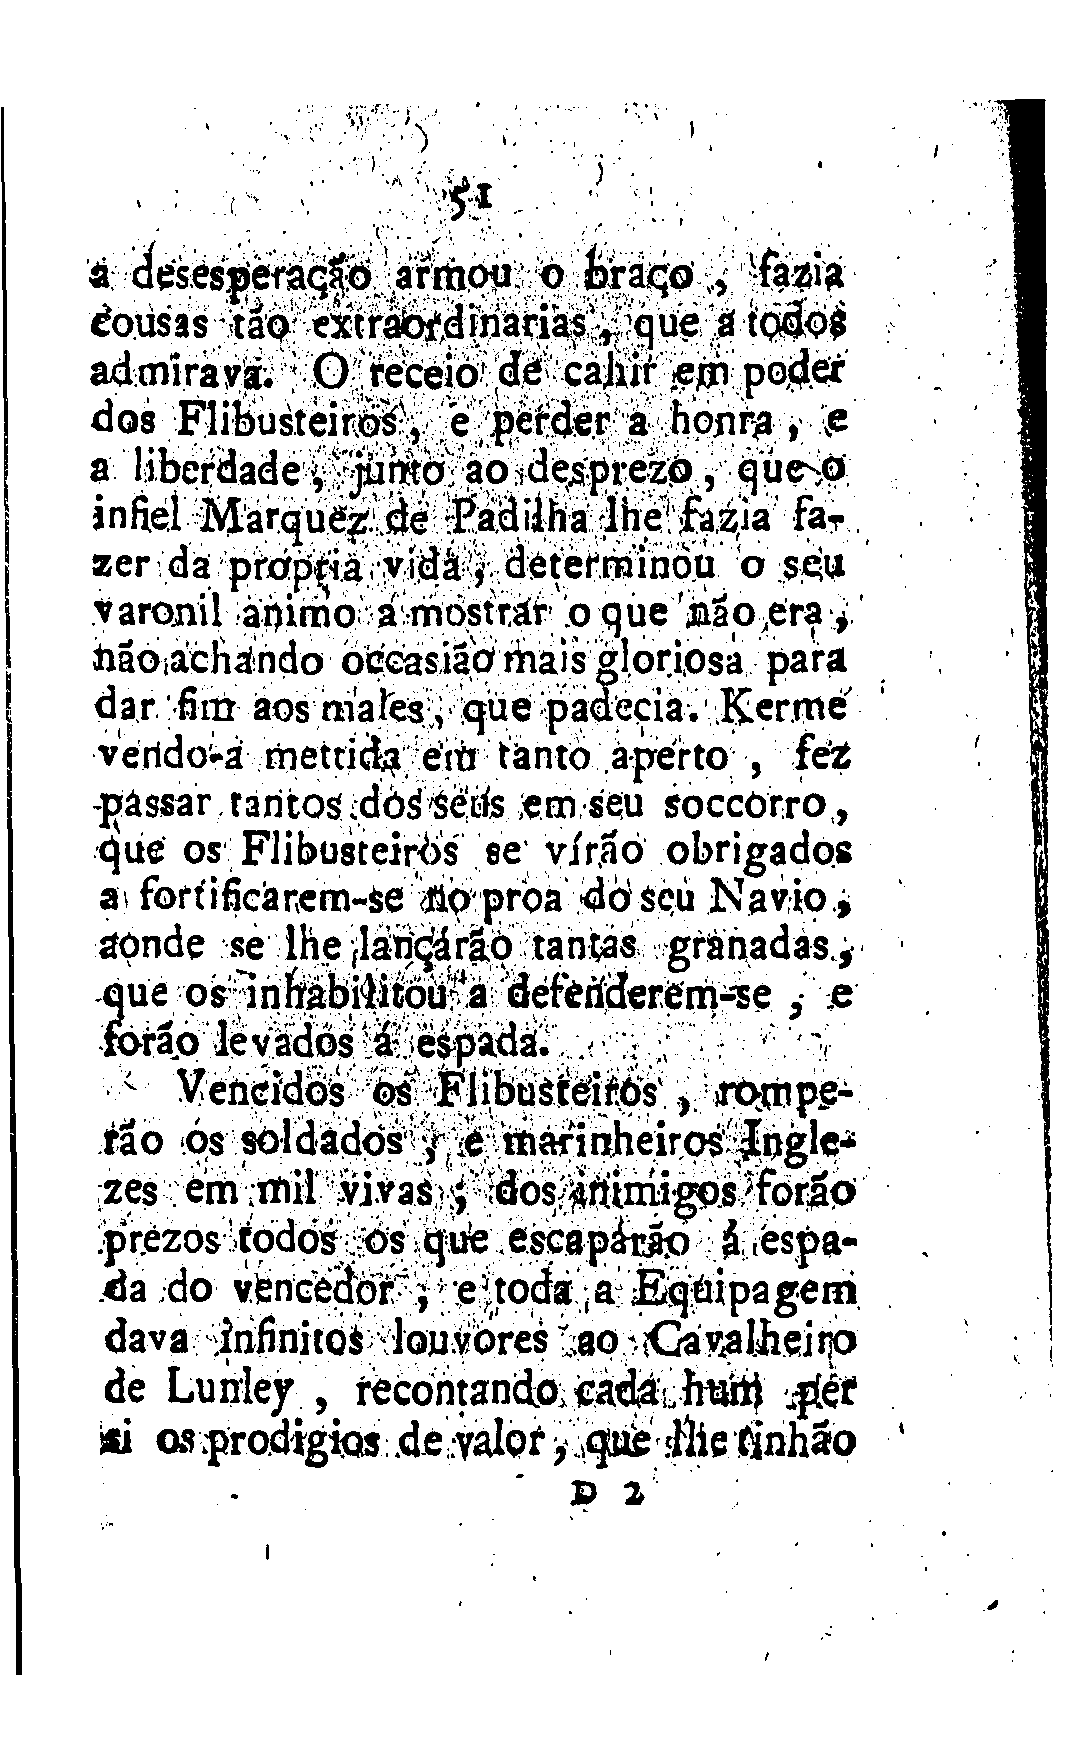
\includegraphics[width=0.55\textwidth]{imagens/amante_p050.png}
    \caption{Exemplo de página difícil: \textit{A Amante Militar}, p.\ 50. Tipografia
    séc.\ XVIII, degradação severa.}
    \label{fig:pagina_dificil}
    \fonte{NUPILL/UFSC.}
\end{figure}

\section{Seleção das Páginas}

Foram selecionadas 20 páginas distribuídas entre as cinco obras, de forma alternada ao
longo de cada volume, de modo a cobrir diferentes seções do texto e evitar viés de
concentração em uma única região do livro. Páginas em branco, páginas de título,
frontispícios e páginas com ilustrações sem texto foram excluídas da seleção. A
distribuição resultou em 5 páginas fáceis, 8 médias e 7 difíceis, com peso maior nas
classes de maior desafio, que são as mais relevantes para a avaliação dos modelos. A
Tabela~\ref{tab:paginas_corpus} apresenta as páginas selecionadas.

\begin{table}[H]
\centering
\caption{Páginas selecionadas para a regra ouro, por obra e classe de dificuldade.}
\label{tab:paginas_corpus}
\renewcommand{\arraystretch}{1.3}
\begin{tabular}{p{4.5cm} c c p{5cm}}
\hline
\textbf{Obra} & \textbf{Pág. PDF} & \textbf{Dificuldade} & \textbf{Características} \\
\hline
\textit{Heloíza}              & 25  & Fácil   & Prosa + poesia, boa qualidade \\
\textit{Heloíza}              & 40  & Fácil   & Prosa densa, tipografia clara \\
\textit{Heloíza}              & 70  & Fácil   & Poesia com múltiplos interlocutores \\
\textit{Heloíza}              & 100 & Fácil   & Poesia com falas e nota de rodapé \\
\textit{Heloíza}              & 130 & Fácil   & Prosa densa, nota de rodapé em itálico \\
\hline
\textit{Culto à Mulher} v.\,1 & 35  & Médio   & Prosa + orações, layout variado \\
\textit{Culto à Mulher} v.\,1 & 80  & Médio   & Poesia esparsa, degradação lateral \\
\textit{Culto à Mulher} v.\,1 & 155 & Médio   & Poesia + data/local no rodapé \\
\textit{Culto à Mulher} v.\,1 & 230 & Médio   & Prosa muito densa, bordas deterioradas \\
\textit{Culto à Mulher} v.\,2 & 20  & Médio   & Poesia densa, tipografia monoespaçada \\
\textit{Culto à Mulher} v.\,2 & 50  & Médio   & Poesia, degradação moderada \\
\textit{Culto à Mulher} v.\,2 & 100 & Médio   & Prosa curta, mancha sobre o texto \\
\textit{Culto à Mulher} v.\,2 & 170 & Médio   & Prosa densa com título de seção \\
\hline
\textit{A Amante Militar}     & 8   & Difícil & Texto denso, tipografia séc.\ XVIII \\
\textit{A Amante Militar}     & 35  & Difícil & Caracteres fundidos, ruído moderado \\
\textit{A Amante Militar}     & 65  & Difícil & Texto contínuo, degradação média \\
\textit{A Amante Militar}     & 95  & Difícil & Prosa densa, alta compactação \\
\textit{O Feliz Independente} & 50  & Difícil & Tipografia séc.\ XVIII, texto narrativo \\
\textit{O Feliz Independente} & 200 & Difícil & Prosa densa, itálico intercalado \\
\textit{O Feliz Independente} & 800 & Difícil & Texto compacto, degradação nas bordas \\
\hline
\end{tabular}
\fonte{Elaborado pelo autor.}
\end{table}

\section{Processo de Transcrição Manual}

A transcrição manual das 20 páginas selecionadas foi realizada pelo próprio autor deste
trabalho. O processo consistiu na leitura direta das imagens digitalizadas e na digitação
fiel do conteúdo textual, respeitando os seguintes critérios:

\begin{itemize}
    \item \textbf{Fidelidade ortográfica}: a ortografia original foi preservada
    integralmente, incluindo grafias arcaicas, acentuação da época e uso de maiúsculas
    não padrão. Nenhuma normalização ortográfica foi aplicada.

    \item \textbf{Preservação de layout textual}: quebras de linha de poemas, recuos de
    parágrafo e separações de seção foram mantidos conforme o original.

    \item \textbf{Tratamento de ambiguidades}: nos casos em que um caractere estava
    ilegível por degradação, a decisão de transcrição foi registrada e submetida à
    validação pelo NUPILL.

    \item \textbf{Exclusão de elementos não textuais}: numeração de página, cabeçalhos
    de volume e ornamentos tipográficos não foram incluídos na transcrição.
\end{itemize}

\section{Validação da Regra Ouro}

As transcrições manuais foram realizadas pelo autor deste trabalho, de 23 anos,
graduando em Ciência da Computação, e serão validadas pelo professor coorientador,
Prof.\ Dr.\ Alckmar Luiz dos Santos, coordenador do NUPILL e especialista em
literatura brasileira histórica. O processo de validação consistirá na comparação
independente entre a transcrição produzida pelo autor e o conteúdo da imagem original,
com foco especial nas passagens ambíguas identificadas durante a transcrição.

As divergências encontradas serão resolvidas por consenso entre o autor e o revisor. O
resultado final é um conjunto de 20 arquivos de texto plano, um por página, que
constituirão a regra ouro utilizada para o cálculo de WER e CER em todos os experimentos
deste trabalho.

%=====================================================================
% CAPÍTULO 5: METODOLOGIA EXPERIMENTAL
%=====================================================================
\chapter{Metodologia Experimental}

\section{Visão Geral}

Este trabalho adota uma abordagem experimental estruturada em cinco fases sequenciais,
orientada pelo objetivo central de identificar e aplicar a técnica de OCR mais adequada
para a digitalização de obras literárias históricas em português. Inicialmente, é
realizada uma avaliação preliminar de diferentes modelos OCR sobre uma amostra
representativa do corpus. Em seguida, seleciona-se o modelo mais adequado com base em
métricas quantitativas e critérios práticos. Após essa etapa, é implementado e
configurado um pipeline de extração automática de texto, posteriormente aplicado ao
corpus completo. Por fim, os textos extraídos são validados qualitativamente e
quantitativamente, e os resultados obtidos são documentados.

A Figura~\ref{fig:metodologia_geral} apresenta uma visão geral das fases da metodologia
proposta neste trabalho.

\begin{figure}[H]
    \centering
    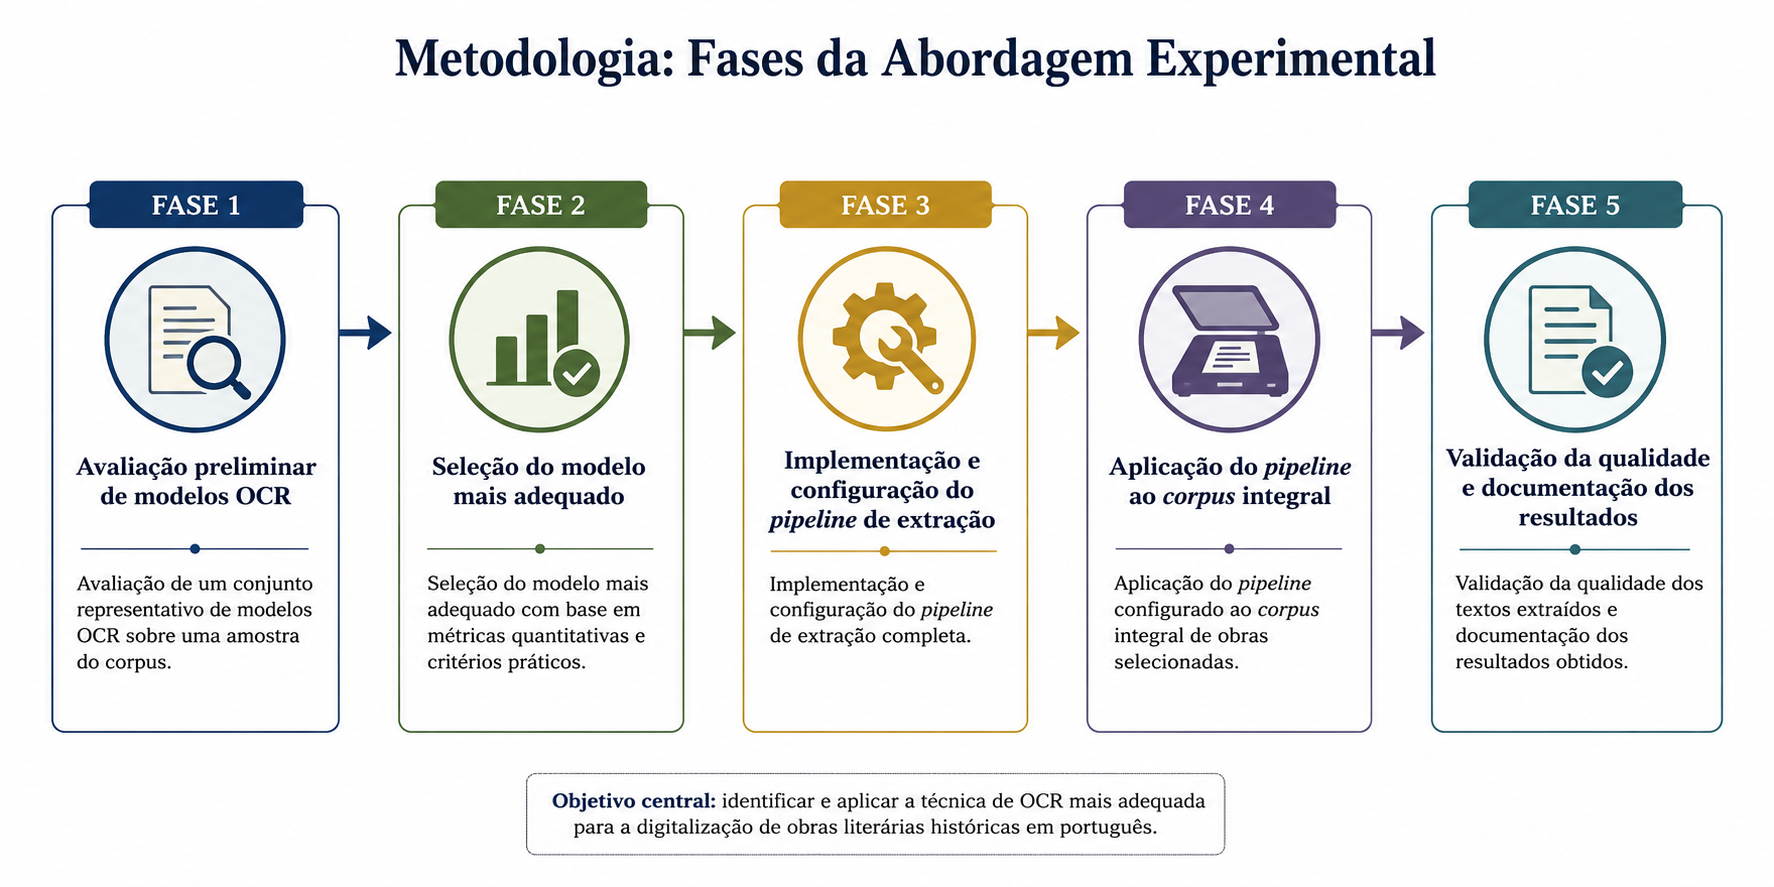
\includegraphics[width=\textwidth]{imagens/fases_metodologia.png}
    \caption{Fases da abordagem experimental proposta para seleção e aplicação de
    técnicas de OCR em obras literárias históricas.}
    \label{fig:metodologia_geral}
\end{figure}

As ferramentas avaliadas neste trabalho, descritas na Seção~\ref{sec:ferramentas}, foram
selecionadas com base em benchmarks recentes da literatura, especialmente os estudos de
Data Unboxed \cite{dataunboxed2025} e Vesalainen et al.\ \cite{vesalainen2025}, que
compararam diferentes abordagens de OCR aplicadas a documentos complexos e históricos.
A seleção contempla representantes das quatro gerações tecnológicas identificadas nesses
trabalhos: OCR clássico, modelos baseados em aprendizado profundo, arquiteturas
Transformer e modelos de linguagem visual (VLMs). Dessa forma, busca-se analisar como
cada abordagem se comporta no contexto específico de obras literárias históricas em
língua portuguesa, cenário ainda pouco explorado nos estudos anteriores.

\clearpage

\section{Fase 1: Configuração e Análise Preliminar dos Modelos}
\label{sec:fase1}

Esta fase consistiu na configuração de todos os modelos candidatos e na execução de
uma avaliação qualitativa inicial sobre uma amostra representativa do corpus. O
objetivo não foi ainda produzir métricas definitivas, mas verificar a viabilidade
operacional de cada ferramenta, identificar dificuldades de instalação e obter uma
primeira impressão visual da qualidade das transcrições produzidas.

\subsection{Amostra de Avaliação Preliminar}

Para a avaliação preliminar, foram selecionadas cinco páginas do corpus, uma por obra,
abrangendo os três níveis de dificuldade definidos no Capítulo~4: a página~40 de
\textit{Heloíza} (fácil), a página~55 de \textit{Culto à Mulher} vol.\,1 (médio), a
página~50 de \textit{Culto à Mulher} vol.\,2 (médio), a página~35 de \textit{A Amante
Militar} (difícil) e a página~200 de \textit{O Feliz Independente} (difícil). Cada
imagem foi extraída do PDF original a 300 DPI e convertida para PNG por meio de um
script Python utilizando a biblioteca \texttt{pdf2image}.

\subsection{Configuração dos Modelos}

\subsubsection{Tesseract 5}

O Tesseract foi instalado via gerenciador de pacotes do sistema operacional
(\texttt{apt install tesseract-ocr tesseract-ocr-por}), incluindo o pacote de dados
de idioma para o português (\texttt{por}). A invocação foi realizada por meio da
biblioteca Python \texttt{pytesseract}, com configuração de página
\texttt{--psm~6} (bloco de texto uniforme) e idioma \texttt{por+eng} para lidar com
eventuais termos em latim presentes nas obras.

\subsubsection{EasyOCR}

O EasyOCR foi instalado via \texttt{pip install easyocr} sem dependências adicionais
além do PyTorch. A inicialização do leitor foi realizada com os idiomas
\texttt{['pt', 'en']}, permitindo reconhecimento bilíngue. A execução utilizou a GPU
disponível, com o parâmetro \texttt{gpu=True}.

\subsubsection{PaddleOCR}

A instalação do PaddleOCR exigiu a instalação prévia do framework PaddlePaddle, que
apresentou incompatibilidades com a versão de CUDA disponível no ambiente, exigindo
a seleção manual de uma versão compatível. Após resolução das dependências, o modelo
foi configurado com \texttt{lang='latin'}, opção mais próxima disponível para o
português no modelo de reconhecimento padrão.

\subsubsection{DocTR}

O DocTR foi instalado via \texttt{pip install python-doctr[torch]}, utilizando o
backend PyTorch. O pipeline foi instanciado com os modelos padrão de detecção
(\texttt{db\_resnet50}) e reconhecimento (\texttt{crnn\_vgg16\_bn}), aplicados
diretamente sobre as imagens PNG sem configuração adicional.

\subsubsection{TrOCR}

As variantes \texttt{base-handwritten} e \texttt{large-handwritten} do TrOCR foram
carregadas a partir do Hugging Face Hub via \texttt{transformers}, utilizando o
processador \texttt{TrOCRProcessor} e o modelo \texttt{VisionEncoderDecoderModel}.
A inferência foi realizada com GPU. Por operar em nível de linha de texto, cada
imagem de página foi previamente segmentada em linhas com o auxílio do
\texttt{craft-text-detector} antes de ser processada pelo modelo.

\subsubsection{VLMs Locais via Ollama}

Os modelos Gemma~4, DeepSeek-VL2 e Qwen2.5-VL foram executados localmente por meio
da plataforma Ollama. Após a instalação do Ollama (\texttt{curl -fsSL
https://ollama.com/install.sh | sh}), cada modelo foi obtido com o comando
\texttt{ollama pull}, sendo utilizadas as variantes de menor tamanho compatíveis com
a memória de vídeo disponível. A interação com os modelos foi realizada via API REST
local (\texttt{http://localhost:11434}), enviando a imagem codificada em base64
junto a um \textit{prompt} instrucional padronizado solicitando a transcrição fiel
do conteúdo da página, sem normalização ortográfica.

\subsubsection{LlamaParse}

O LlamaParse foi acessado via API, utilizando a biblioteca oficial
\texttt{llama-parse}. Foi avaliado em duas configurações: modo \textit{Cost Effective}
(básico) e modo \textit{Agentic}. A autenticação foi realizada por meio de chave de
API obtida no portal da LlamaIndex. As páginas foram enviadas como arquivos PDF
individuais.

\subsubsection{Mistral OCR}

O Mistral OCR foi acessado via API REST, utilizando a biblioteca \texttt{mistralai}
para Python. Cada imagem foi enviada codificada em base64, e a resposta continha o
texto transcrito em formato estruturado. A autenticação foi realizada por chave de
API.

\subsubsection{Gemini 2.0 Flash}

O Gemini 2.0 Flash foi acessado via API do Google, utilizando a biblioteca
\texttt{google-generativeai}. As imagens foram enviadas diretamente como parte do
conteúdo multimodal da requisição, acompanhadas de um \textit{prompt} instrucional
idêntico ao utilizado nos demais VLMs.

\subsection{Observações Qualitativas}

A inspeção visual das transcrições produzidas na amostra preliminar permitiu
identificar padrões de comportamento distintos entre as categorias de modelos. Os
modelos clássicos e baseados em CRNN apresentaram dificuldades crescentes conforme
o nível de degradação e a complexidade tipográfica das páginas, sendo os erros mais
frequentes a confusão entre caracteres visualmente similares (e.g., \texttt{rn} por
\texttt{m}, \texttt{l} por \texttt{I}) e a falha na segmentação de linhas em layouts
com múltiplas colunas. Os modelos Transformer (TrOCR) produziram transcrições mais
coesas em páginas de dificuldade baixa e média, mas apresentaram erros de alucinação
em páginas com degradação severa, provavelmente associados à falta de dados históricos
em português no treinamento. Os VLMs demonstraram maior robustez ao layout e à
degradação, porém com tendência observada de modernização de grafias arcaicas,
conforme reportado por Vesalainen et al.\ \cite{vesalainen2025}.

\begin{figure}[H]
    \centering
    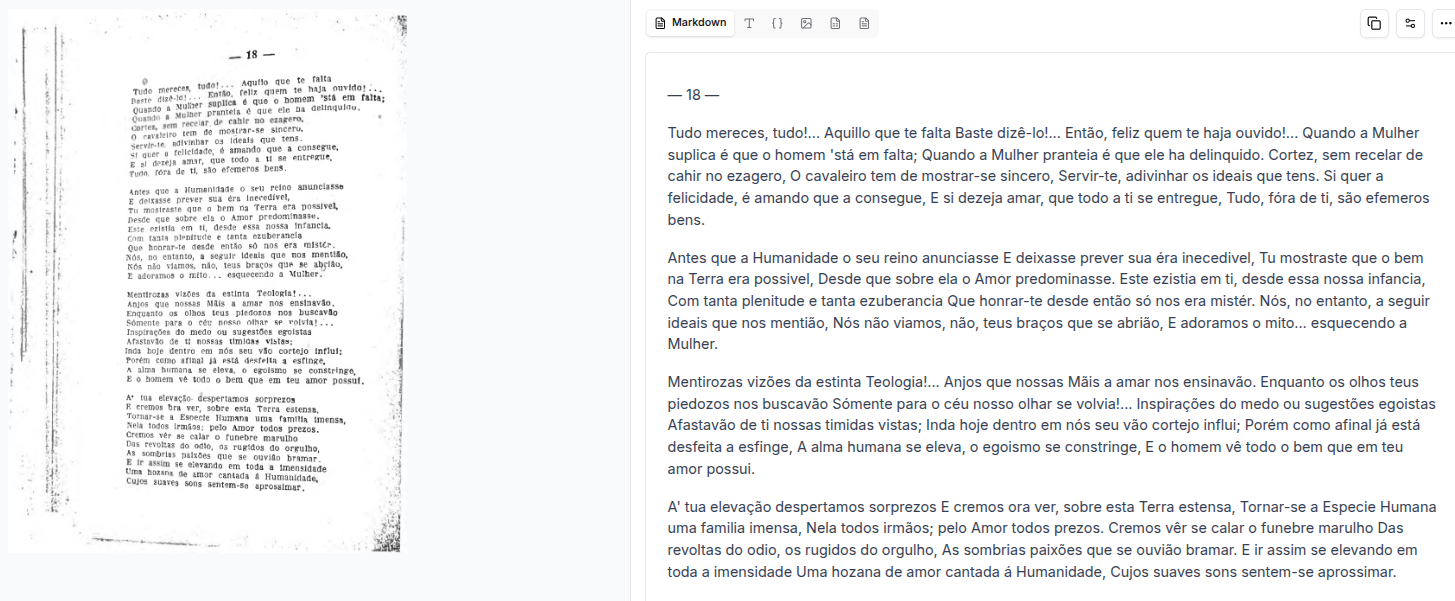
\includegraphics[width=\textwidth]{imagens/culto_p018_original.png}
    \caption{Exemplo de par entrada/saída de OCR. \textbf{Esquerda:} página~18 de
    \textit{Culto à Mulher} vol.\,1, \textbf{Direita (trecho):} saída do modelo LlamaParse (agentic mode)}
    \label{fig:exemplo_ocr_par}
    \fonte{NUPILL/UFSC (imagem); elaborado pelo autor (transcrição OCR).}
\end{figure}

\FloatBarrier

\section{Fase 2: Seleção do Modelo}
\label{sec:fase2}

Concluída a avaliação preliminar, procedeu-se à seleção do modelo a ser utilizado no
pipeline de extração completa. A seleção foi estruturada em duas etapas: primeiro, uma
triagem por critérios práticos eliminou modelos inviáveis para o contexto deste trabalho;
em seguida, entre os modelos remanescentes, a decisão foi fundamentada em desempenho
reportado na literatura e adequação ao corpus.

\subsection{Critérios de Triagem}

Três critérios foram aplicados sequencialmente para eliminar modelos antes da comparação
de desempenho:

\begin{enumerate}
    \item \textbf{Custo financeiro}: modelos via API com custo elevado por página foram
    descartados quando alternativas gratuitas apresentavam desempenho competitivo nos
    benchmarks da literatura. O modo \textit{Agentic} do LlamaParse, com custo de
    US\$\,0,0125 por página, foi eliminado nesta etapa, uma vez que o modo básico
    (\textit{Cost Effective}) oferece resultado similar a custo oito vezes menor, e VLMs
    locais gratuitos superam ambos em benchmarks recentes \cite{dataunboxed2025}.

    \item \textbf{Custo computacional}: modelos com demanda de GPU incompatível com o
    hardware disponível ou com tempo de inferência proibitivo foram descartados. A
    variante \texttt{large} do TrOCR foi eliminada nesta etapa por exigir
    significativamente mais memória de vídeo que a variante \texttt{base} sem ganho
    proporcional de desempenho em documentos históricos \cite{vesalainen2025}.

    \item \textbf{Desempenho em documentos históricos}: modelos sem resultados
    reportados em benchmarks de documentos históricos ou com desempenho consistentemente
    inferior foram descartados.
\end{enumerate}

\subsection{Quadro Comparativo para Seleção}

A Tabela~\ref{tab:selecao_modelos} apresenta os modelos remanescentes após a triagem,
comparados segundo custo, requisito de GPU, CER e WER médios reportados em benchmarks
recentes da literatura, e adequação ao contexto deste trabalho.

\FloatBarrier
\begin{table}[H]
\centering
\caption{Comparativo dos modelos candidatos para seleção, com base em critérios práticos
e desempenho reportado na literatura.}
\label{tab:selecao_modelos}
\renewcommand{\arraystretch}{1.4}
{\small
\begin{tabular}{p{2.4cm} p{1.5cm} p{2cm} p{1.4cm} p{1.4cm} p{4.5cm}}
\hline
\textbf{Modelo} & \textbf{Custo} & \textbf{GPU} & \textbf{CER\,(\%)} &
\textbf{WER\,(\%)} & \textbf{Observação} \\
\hline
Tesseract 5
  & Gratuito & Não
  & $\sim$30--50 & $\sim$45--65
  & Referência clássica; degrada com tipografia histórica \\
\hline
EasyOCR
  & Gratuito & Opcional
  & $\sim$20--35 & $\sim$35--55
  & Instalação simples; limitado em layouts complexos \\
\hline
PaddleOCR
  & Gratuito & Opcional
  & $\sim$18--32 & $\sim$30--50
  & Incompatibilidades de CUDA na instalação \\
\hline
DocTR
  & Gratuito & Opcional
  & $\sim$18--30 & $\sim$30--48
  & Pipeline moderno; sem modelo específico para português \\
\hline
TrOCR \texttt{base}
  & Gratuito & Recomenda
  & $\sim$12--25 & $\sim$22--40
  & Melhor Transformer avaliado; sensível a degradação severa
  \cite{vesalainen2025} \\
\hline
Gemma~4
  & Gratuito & Recomenda
  & $\sim$8--18 & $\sim$15--30
  & VLM local recente; poucos benchmarks em documentos históricos \\
\hline
DeepSeek-VL2
  & Gratuito & Recomenda
  & $\sim$8--20 & $\sim$15--32
  & Arquitetura MoE eficiente; poucos dados em português histórico \\
\hline
\textbf{Qwen2.5-VL}
  & \textbf{Gratuito} & \textbf{Recomenda}
  & $\boldsymbol{\sim}$\textbf{5--12} & $\boldsymbol{\sim}$\textbf{10--22}
  & \textbf{Melhor desempenho em documentos históricos; projetado para
  documentos \cite{vesalainen2025}} \\
\hline
LlamaParse Basic
  & Pago & Não
  & $\sim$6--14 & $\sim$12--25
  & Competitivo, mas custo por página e envio de dados a terceiros \\
\hline
Mistral OCR
  & Pago & Não
  & $\sim$5--12 & $\sim$10--20
  & Desempenho comparável ao Qwen2.5-VL, porém com custo financeiro \\
\hline
Gemini 2.0 Flash
  & Pago & Não
  & $\sim$5--10 & $\sim$9--18
  & Alto desempenho; descontinuado em jun./2026 \cite{gemini_pricing} \\
\hline
\end{tabular}
\fonte{Valores de CER e WER adaptados de \cite{vesalainen2025,dataunboxed2025};
demais colunas elaboradas pelo autor.}
\end{table}
}
\FloatBarrier

\subsection{Modelo Selecionado e Justificativa}

Com base na triagem e no comparativo da Tabela~\ref{tab:selecao_modelos}, foi
selecionado o \textbf{Qwen2.5-VL}, executado localmente via Ollama, como modelo para
compor o pipeline de extração. A escolha considera tanto o desempenho obtido em
trabalhos recentes quanto aspectos práticos relacionados à implantação da solução.

Em benchmarks voltados a documentos históricos impressos, o Qwen2.5-VL apresenta os
menores valores de CER e WER entre os modelos gratuitos avaliados, superando com ampla
margem os motores clássicos e as arquiteturas baseadas em CRNN, e alcançando resultados
próximos aos de serviços comerciais disponibilizados via API \cite{vesalainen2025}.
Além disso, sua arquitetura, baseada em um Vision Transformer de resolução dinâmica,
foi projetada para lidar com documentos de estrutura complexa, incluindo múltiplas
colunas, diferentes estilos tipográficos e elementos de layout variados, características
presentes nas obras utilizadas neste trabalho \cite{qwen2025vl}.

Outro fator relevante é a possibilidade de execução local por meio do Ollama. Essa
abordagem elimina custos por página processada e evita o envio das imagens do acervo
do NUPILL para serviços externos, favorecendo tanto a sustentabilidade financeira
quanto o controle sobre os dados da pesquisa. Soma-se a isso o fato de o modelo estar
disponível sob licença Apache~2.0, permitindo que o pipeline proposto possa ser
reproduzido por outros pesquisadores sem dependência de serviços proprietários ou chaves
de acesso a APIs.

Apesar dessas vantagens, o modelo apresenta uma limitação já apontada na literatura.
Vesalainen et al.\ \cite{vesalainen2025} identificaram que modelos de visão-linguagem
podem modernizar automaticamente grafias históricas durante a transcrição, alterando de
forma silenciosa a escrita original do documento. Como a preservação da ortografia é um
requisito deste trabalho, esse comportamento será monitorado durante a etapa de
validação, por meio de análise específica de grafias históricas e caracteres
potencialmente sensíveis.

\section{Fase 3: Implementação do Pipeline de Extração}
\label{sec:fase3}

Com o modelo selecionado, a terceira fase consiste na implementação de um pipeline
automatizado de extração de texto, capaz de processar em lote todas as páginas do
corpus. O pipeline é estruturado em quatro etapas sequenciais, ilustradas na
Figura~\ref{fig:pipeline_extracao}: conversão das páginas do PDF em imagens, envio
de cada imagem ao modelo OCR, coleta e normalização da transcrição produzida, e
armazenamento estruturado dos resultados.

\begin{figure}[H]
    \centering
    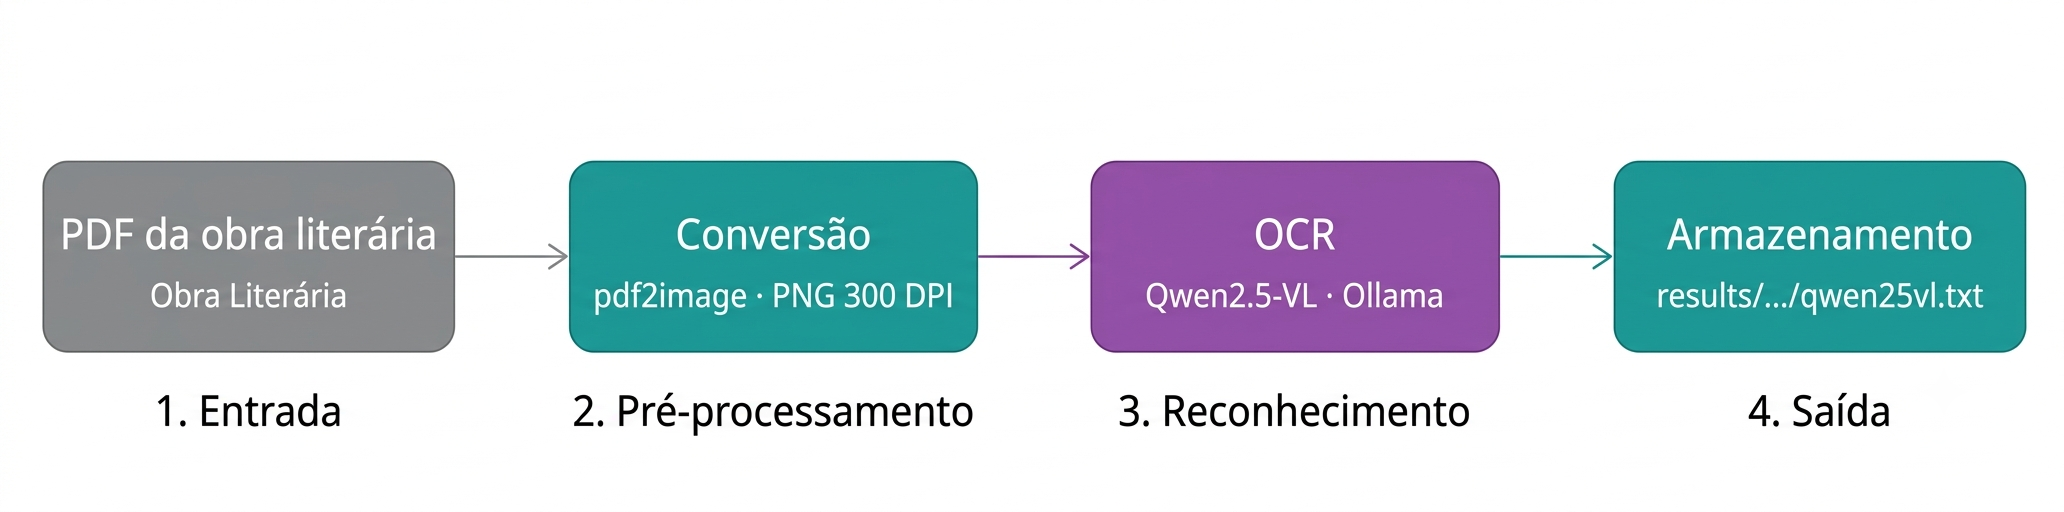
\includegraphics[width=\textwidth]{imagens/pipeline_extracao.png}
    \caption{Pipeline de extração automática de texto}
    \label{fig:pipeline_extracao}
    \fonte{Elaborado pelo autor.}
\end{figure}

Cada volume do corpus é convertido página a página em imagens PNG
a 300 DPI, utilizando a biblioteca \texttt{pdf2image}. Cada imagem então
é enviada ao Qwen2.5-VL via API REST local do Ollama, acompanhada de um
\textit{prompt} instrucional padronizado que solicita a transcrição fiel do conteúdo,
explicitando a preservação de grafias históricas e a exclusão de elementos não textuais
como numeração de página e ornamentos tipográficos. Por fim, a resposta do
modelo é coletada e o texto extraído é salvo em arquivo \texttt{.txt} plano, um por
página, seguindo a estrutura de diretórios
\texttt{data/results/\{livro\}/\{pagina\}/qwen25vl.txt}.


A implementação será realizada em Python, organizada como um pacote com uma classe
base abstrata \texttt{BaseOCR} e adaptadores específicos para cada modelo, garantindo
que o pipeline possa ser estendido para outros modelos em trabalhos futuros. 

% ---------------------------------------------------------------
% Fases 4–5: a serem desenvolvidas no TCC2
% ---------------------------------------------------------------

% \section{Fase 4: Validação em Amostra}
% \section{Fase 5: Extração Completa do Corpus}

%=====================================================================
% CAPÍTULOS 6 E 7: A SEREM DESENVOLVIDOS NO TCC2
%=====================================================================

% \chapter{Implementação e Resultados}
% \chapter{Discussão}

%=====================================================================
% CAPÍTULO 8: CONCLUSÃO
%=====================================================================
\chapter{Conclusão}

% Texto introdutório e demais seções a serem desenvolvidos no TCC2.

\section{Trabalhos Futuros}

Com base na revisão bibliográfica realizada, na construção da regra ouro e na
configuração e avaliação preliminar dos modelos, os seguintes trabalhos estão previstos
para a continuação desta pesquisa:

\begin{enumerate}

    \item Implementação e configuração do pipeline de extração automática de texto
    com o modelo selecionado, incluindo script Python com interface de linha de comando,
    logging e tratamento de erros.

    \item Aplicação do pipeline ao corpus completo das obras do NUPILL, com
    documentação dos resultados e estimativa de taxa de erro em larga escala.

    \item Validação qualitativa e quantitativa dos textos extraídos, com análise de
    padrões de erro sistemáticos e recomendações para pós-processamento.

    \item Documentação do processo na forma de diretrizes metodológicas replicáveis,
    orientadas a iniciativas similares de digitalização de acervos históricos em
    português.
\end{enumerate}

%=====================================================================
% ELEMENTOS PÓS-TEXTUAIS
%=====================================================================
\postextual

%=====================================================================
% REFERÊNCIAS BIBLIOGRÁFICAS
% Ordenadas por ordem de primeira aparição no texto (ABNT NBR 6023)
%=====================================================================
\bibliographystyle{abntex2-num}
\bibliography{referencias}

\end{document}